\documentclass[aspectratio=169]{beamer}

\usetheme{default}
\usepackage[utf8]{inputenc}
\usepackage[brazil]{babel}
\usepackage{tikz}
\usepackage{tabularx}
\usetikzlibrary{positioning,shapes.geometric,arrows.meta}
\usepackage{amsmath}
\usepackage{booktabs}
\usepackage{multirow}
\usepackage{graphicx}
\usepackage{hyperref}
\usepackage{amssymb}
\usepackage{colortbl}

% logos em presentation/imgs; figuras desta apresentação em ./figuras
\graphicspath{{../}{figuras/}}

\setbeamertemplate{footline}[frame number]
\setbeamertemplate{frametitle}[default][center]

\mode<presentation>{
\usetheme{Dresden}
\usecolortheme{seagull}
}

\setbeamertemplate{headline}{}

\definecolor{peeblue}{RGB}{1,123,165}
\definecolor{darkblue}{RGB}{0,65,115}
\definecolor{greenwin}{RGB}{0,130,50}

\setbeamercolor*{palette primary}{fg=black,bg=peeblue!80}
\setbeamercolor*{palette secondary}{fg=black,bg=peeblue!80!gray!80}
\setbeamercolor*{palette tertiary}{fg=black,bg=peeblue!100}
\setbeamercolor*{palette quaternary}{fg=black,bg=peeblue!110}

\usebackgroundtemplate
{%
    \begin{picture}(210,40)(-5,2)
    
\includegraphics[width=0.07\paperwidth,keepaspectratio]{imgs/pee-logo-short.png}
    \end{picture}%
}

\title{Reconhecimento Acústico de Alvos Submarinos no Dataset IARA}
\subtitle{A Classe SMALL: o Que Sabemos Até Agora}
\author{Evandro Rocha}
\date{Novembro de 2026}

\institute
{
  Universidade Federal do Rio de Janeiro\\
  UFRJ / COPPE / PEE
}

\newcommand{\cahi}[1]{\cellcolor{green!30}\textbf{#1}}
\newcommand{\calo}[1]{\cellcolor{red!20}#1}
\newcommand{\camd}[1]{\cellcolor{yellow!35}#1}

\begin{document}

%===========================================
% CAPA
%===========================================
{
\usebackgroundtemplate{
    \begin{picture}(210,55)(-5,0)
    
\includegraphics[height=0.14\paperwidth,keepaspectratio]{imgs/pee-logo.png}
    \end{picture}%
    \begin{picture}(210,55)(-28,2)
    
\includegraphics[height=0.14\paperwidth,keepaspectratio]{imgs/coppe-logo.pdf}
    \end{picture}
}
\begin{frame}
  \bigskip\bigskip\bigskip\bigskip
  \titlepage
\end{frame}
}

%===========================================
% AGENDA
%===========================================
\begin{frame}{Agenda da Apresentação}
  \footnotesize
  \setbeamercolor{block title}{bg=darkblue,fg=white}
  \setbeamercolor{block body}{bg=peeblue!8,fg=black}
  \setbeamertemplate{section in toc}{%
    \vspace{0.14cm}%
    \leavevmode%
    \tikz[baseline=-0.65ex]\node[circle,fill=peeblue,text=white,inner sep=0pt,font=\tiny\bfseries,minimum size=1.35em]{\inserttocsectionnumber};%
    \hspace{0.35em}%
    \inserttocsection\par%
  }
  \begin{columns}[t]
      \begin{column}{0.48\textwidth}
          \begin{block}{\small\textbf{I. Dados e Extrações}}
              \tableofcontents[sections={1-3}]
          \end{block}
      \end{column}
      \begin{column}{0.48\textwidth}
          \begin{block}{\small\textbf{II. O Que o Som da Classe SMALL Mostra}}
              \tableofcontents[sections={4-8}]
          \end{block}
      \end{column}
  \end{columns}
\end{frame}

%===========================================
% RESUMO
%===========================================
\begin{frame}{Resumo}
    \footnotesize
    \begin{block}{\small Pergunta: existe uma assinatura acústica própria da classe SMALL?}
        \scriptsize
        \begin{enumerate}
            \setlength{\itemsep}{2pt}
            \item \textbf{SMALL é, na prática, ``lancha de prático''.} 476 gravações de 87 navios, mas 5 lanchas somam 59\%: equivale a \textbf{$\sim$12 navios} igualmente gravados.
            \item \textbf{No IARA, tipo e tamanho são a mesma coisa.} Lanchas, rebocadores e pesca são SMALL; apoio offshore é MEDIUM; mercantes são LARGE. O IARA não separa ``som de barco pequeno'' de ``som desses tipos''.
            \item \textbf{O modelo acerta $\sim$50\% das SMALL de navios nunca vistos}, por igual em lanchas, rebocadores e pesca. Os erros vão para MEDIUM ($\sim$23\%) e para LARGE ($\sim$24\%).
            \item \textbf{Nenhuma assinatura positiva de SMALL} no LOFAR, no DEMON, no MEL nem no HHT. O SMALL é reconhecido pela \textbf{falta} do que o LARGE tem: grave forte em 31--86 Hz e linha DEMON forte e grave.
            \item \textbf{SMALL e MEDIUM são iguais} em todas as medidas testadas.
            \item \textbf{SMALL $\to$ LARGE:} gravações com o grave de 31--86 Hz no nível das LARGE (inclusive dentro da mesma lancha).
            \item \textbf{Próximo passo:} testar ``tamanho dentro do mesmo tipo'' numa base com mais navios (UniqueShip: 286 rebocadores de 10 a 50 m) e pedir ao PMPAS-BS gravações mais recentes, com mais diversidade de navios.
        \end{enumerate}
    \end{block}
\end{frame}

%===========================================
% SEÇÃO 1 - DATASET
%===========================================
\section{O Dataset IARA}

\begin{frame}
    \centering
    \huge O Dataset IARA
\end{frame}

\begin{frame}{O IARA em Números}
    \footnotesize
    \begin{columns}[T]
        \begin{column}{0.44\textwidth}
            \begin{block}{\small Origem}
                \scriptsize
                \begin{itemize}
                    \setlength{\itemsep}{1pt}
                    \item Monitoramento da Bacia de Santos (PMPAS-BS, Petrobras): \textbf{1.825 gravações, 129 h 34 min}, de 2 a 5 min.
                    \item Observatórios fixos no fundo (19--28 m), \textbf{48 kHz, 16 bits}, resposta plana até 20 kHz.
                    \item Rótulo pelo AIS: \textbf{um só navio} na inclusão e nenhum outro a menos de 2 km; verificação acústica e manual.
                    \item Classe pelo \textbf{comprimento}: SMALL $<$ 50 m; MEDIUM 50--100 m; LARGE $\geq$ 100 m.
                    \item \textbf{Não há} distância por gravação, data, observatório nem calibração.
                \end{itemize}
            \end{block}
        \end{column}
        \begin{column}{0.54\textwidth}
            \centering
            \scriptsize
            \textbf{Subconjuntos usados (observatórios fixos)}\\[3pt]
            \tiny\setlength{\tabcolsep}{3pt}
            \begin{tabular}{@{}lccrrrr@{}}
                \toprule
                Sub. & Inclusão & CPA & SMALL & MEDIUM & LARGE & BG \\
                \midrule
                A & $\leq$ 250 m & sim & 113 & 120 & 223 & -- \\
                B & $\leq$ 250 m & não & 90 & 73 & 36 & -- \\
                C & 250--500 m & sim & 104 & 75 & 162 & -- \\
                D & 250--500 m & não & 169 & 129 & 151 & -- \\
                E & -- & -- & -- & -- & -- & 261 \\
                \midrule
                \textbf{Total} & & & \textbf{476} & \textbf{397} & \textbf{572} & \textbf{261} \\
                \bottomrule
            \end{tabular}\\[4pt]
            \scriptsize
            \begin{itemize}
                \setlength{\itemsep}{1pt}
                \item \textbf{CPA} = ponto de maior aproximação; sem CPA (B, D), o navio entra ou sai da região durante a gravação.
                \item BACKGROUND: sem navio a menos de 10 km, \textbf{todo} no subconjunto E (comparar com ele mistura classe com equipamento).
            \end{itemize}
        \end{column}
    \end{columns}
\end{frame}

\begin{frame}{CPA e Distância: Como as Gravações de Navio Foram Selecionadas}
    \footnotesize
    \begin{columns}[T]
        \begin{column}{0.44\textwidth}
            \centering
            \vspace{0.25cm}
            \begin{tikzpicture}[scale=0.52, every node/.style={font=\tiny}]
                % regiões
                \fill[peeblue!8] (0,0) circle (3.0);
                \fill[peeblue!22] (0,0) circle (1.5);
                \draw[peeblue!70, dashed] (0,0) circle (3.0);
                \draw[peeblue!70, dashed] (0,0) circle (1.5);
                \node[peeblue!80!black] at (-0.75,0.75) {250 m};
                \node[peeblue!80!black] at (-1.95,1.6) {500 m};
                % hidrofone
                \fill[black] (0,0) circle (0.11);
                \node[above right] at (0.02,0.02) {hidrofone};
                % rota 1: passa a ~150 m (A ou B)
                \draw[-{Stealth[length=5pt]}, thick, greenwin] (-3.9,-0.9) -- (3.9,-0.9);
                \fill[greenwin] (0,-0.9) circle (0.09);
                \draw[greenwin, densely dotted] (0,0) -- (0,-0.9);
                \node[greenwin, left] at (-0.05,-0.55) {CPA};
                \node[greenwin, anchor=west] at (2.3,-1.25) {A ou B};
                % rota 2: passa a ~350 m (C ou D)
                \draw[-{Stealth[length=5pt]}, thick, orange] (-3.9,2.1) -- (3.9,2.1);
                \fill[orange] (0,2.1) circle (0.09);
                \node[orange, above] at (0.75,2.1) {CPA};
                \node[orange, anchor=west] at (2.3,2.45) {C ou D};
                % rota 3: passa a ~1 km (fora)
                \draw[-{Stealth[length=5pt]}, thick, gray] (-3.9,3.55) -- (3.9,3.55);
                \node[gray, anchor=west] at (1.3,3.85) {a 1 km: fora do IARA (A--E)};
            \end{tikzpicture}\\[2pt]
            \scriptsize
            \setlength{\tabcolsep}{4pt}
            \begin{tabular}{@{}lcc@{}}
                \toprule
                & Tem o CPA & Não tem o CPA \\
                \midrule
                até 250 m & \textbf{A} & \textbf{B} \\
                250--500 m & \textbf{C} & \textbf{D} \\
                \bottomrule
            \end{tabular}
        \end{column}
        \begin{column}{0.54\textwidth}
            \begin{block}{\small O que é o CPA}
                \scriptsize
                \textit{Closest Point of Approach}: o \textbf{ponto da rota do navio mais perto do hidrofone} e o instante em que ele passa por ali. O hidrofone fica parado no fundo; o navio se aproxima, passa pelo CPA e se afasta, então a distância muda ao longo da gravação e o som costuma ser mais forte no CPA.
            \end{block}
            \begin{block}{\small Como a distância define o subconjunto}
                \scriptsize
                \begin{itemize}
                    \setlength{\itemsep}{1pt}
                    \item Raio medido \textbf{até o hidrofone}, pelo AIS: \textbf{A e B} = navio a até 250 m; \textbf{C e D} = entre 250 e 500 m.
                    \item \textbf{A e C:} a gravação inclui o CPA. \textbf{B e D:} foi cortada antes ou depois dele (outro navio entraria a menos de 2 km).
                \end{itemize}
            \end{block}
        \end{column}
    \end{columns}
\end{frame}

\begin{frame}{Distância: o Que Fica de Fora e Por Que Importa}
    \footnotesize
    \begin{columns}[T]
        \begin{column}{0.49\textwidth}
            \begin{block}{\small Critérios dos observatórios fixos}
                \scriptsize
                \centering
                \setlength{\tabcolsep}{4pt}
                \begin{tabular}{@{}ll@{}}
                    \toprule
                    Uso & Critério (pelo AIS) \\
                    \midrule
                    Navio, A e B & até 250 m do hidrofone \\
                    Navio, C e D & de 250 a 500 m \\
                    Exclusão (A--D) & nenhum \textbf{outro} navio $<$ 2 km \\
                    BACKGROUND (E) & nenhum navio $<$ 10 km \\
                    \bottomrule
                \end{tabular}
            \end{block}
            \begin{block}{\small O que fica de fora}
                \scriptsize
                \begin{itemize}
                    \setlength{\itemsep}{1pt}
                    \item Navio que passa a 1 km: \textbf{não entra} em A--D, nem em E. Passagens distantes só existem nos dados de \textit{glider} (F, G; inclusão até 10 km), que não usamos.
                    \item Todas as nossas gravações de navio são de passagens a \textbf{até 500 m}.
                \end{itemize}
            \end{block}
        \end{column}
        \begin{column}{0.49\textwidth}
            \begin{block}{\small O que o IARA não informa}
                \scriptsize
                \begin{itemize}
                    \setlength{\itemsep}{1pt}
                    \item A \textbf{distância exata}: só a faixa. Cada passagem tem o seu CPA (80 m, 200 m, 400 m\ldots), e a distância muda ao longo da gravação.
                    \item Qual observatório (hidrofone) gravou cada arquivo.
                \end{itemize}
            \end{block}
            \begin{alertblock}{\small Por que importa para o SMALL}
                \scriptsize
                \begin{itemize}
                    \setlength{\itemsep}{1pt}
                    \item Barco pequeno perto e navio maior longe podem chegar com intensidade parecida.
                    \item O grave do LARGE depende do CPA (pico em 31--86 Hz: 69--76\% com CPA, 33--55\% sem); sem CPA, o LARGE parece um navio menor.
                    \item Lanchas de prático: o pior subconjunto é o \textbf{B} (perto, sem CPA), com 59\% de erradas.
                \end{itemize}
            \end{alertblock}
        \end{column}
    \end{columns}
\end{frame}

\begin{frame}{A Classe SMALL: Poucos Navios Dominam}
    \footnotesize
    \begin{columns}[T]
        \begin{column}{0.55\textwidth}
            \centering
            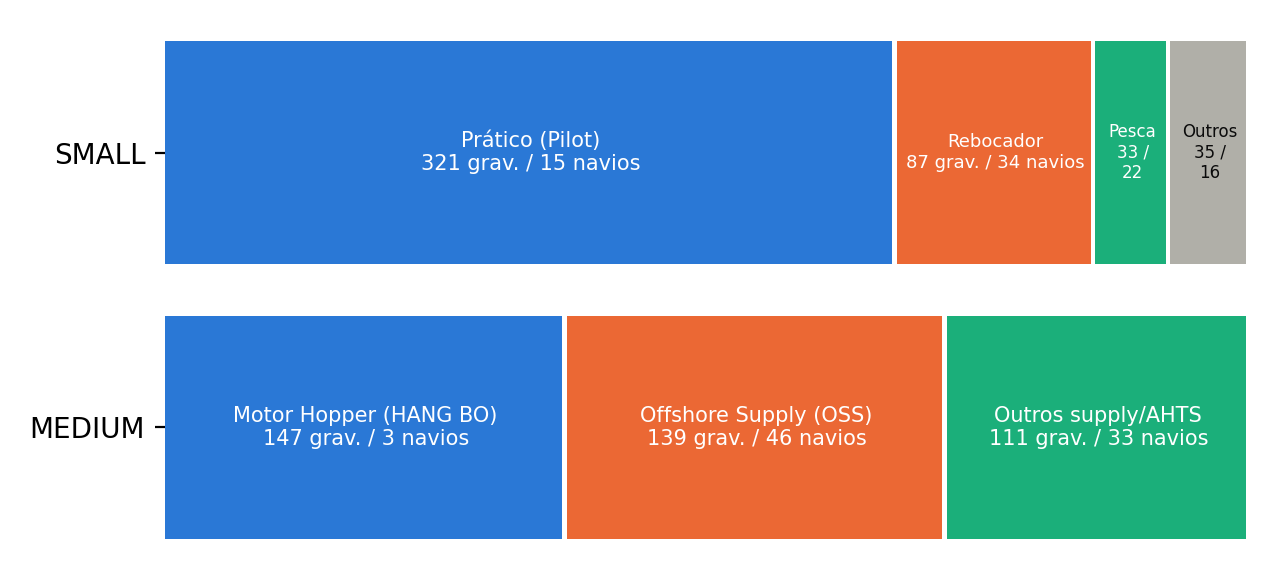
\includegraphics[width=0.92\textwidth]{composicao_tipos.png}\\[4pt]
            \tiny
            \begin{tabular}{@{}lrrc@{}}
                \toprule
                Tipo (SMALL) & Grav. & Navios & Comprimento (25--75\%) \\
                \midrule
                Lancha de prático & 321 & 15 & 11--12 m \\
                Rebocador & 87 & 34 & 25--32 m \\
                Pesca & 33 & 22 & 18--22 m \\
                Outros & 35 & 16 & -- \\
                \bottomrule
            \end{tabular}
        \end{column}
        \begin{column}{0.43\textwidth}
            \begin{block}{\small Leitura}
                \scriptsize
                \begin{itemize}
                    \setlength{\itemsep}{2pt}
                    \item \textbf{5 lanchas de prático} (PILOT 08, 09, 10, 11, 14) somam \textbf{279 das 476 gravações} (59\%).
                    \item \textbf{Nº efetivo de navios} (1/$\Sigma p^2$): SMALL $\approx$ 12, MEDIUM $\approx$ 13, LARGE $\approx$ 214.
                    \item Rebocadores e pesca têm muitos navios, mas \textbf{1--3 gravações cada}.
                    \item Dentro de cada tipo, o comprimento \textbf{quase não varia}: não dá para testar ``tamanho dentro do tipo'' no IARA.
                \end{itemize}
            \end{block}
        \end{column}
    \end{columns}
\end{frame}

\begin{frame}{No IARA, Tipo de Navio e Classe São Quase a Mesma Coisa}
    \footnotesize
    \begin{columns}[T]
        \begin{column}{0.48\textwidth}
            \centering
            \scriptsize
            \textbf{Navios distintos por tipo e classe}\\[3pt]
            \setlength{\tabcolsep}{3pt}
            \begin{tabular}{@{}lrrr@{}}
                \toprule
                Tipo & SMALL & MEDIUM & LARGE \\
                \midrule
                Rebocador & \cahi{34} & 1 & 0 \\
                Pesca & \cahi{22} & 1 & 0 \\
                Lancha de prático & \cahi{15} & 0 & 0 \\
                Offshore Supply & 3 & \cahi{46} & 0 \\
                Outros de apoio offshore & 0 & \cahi{$\sim$30} & 0 \\
                Carga e petroleiros & 0 & 2 & \cahi{$\sim$400} \\
                \bottomrule
            \end{tabular}
        \end{column}
        \begin{column}{0.50\textwidth}
            \begin{block}{\small Consequência}
                \scriptsize
                \begin{itemize}
                    \setlength{\itemsep}{2pt}
                    \item SMALL = \textbf{lancha, rebocador, pesca}; MEDIUM = \textbf{apoio offshore}; LARGE = \textbf{mercante}.
                    \item Só o tipo de navio já separaria SMALL de MEDIUM com AUC 0,98.
                    \item O único tipo presente nas duas classes é o Offshore Supply (3 $\times$ 46): dentro dele o modelo dá AUC 0,62, p = 0,5 (nada).
                    \item \textbf{Qualquer pista que o modelo aprenda para SMALL pode ser ``som de lancha/rebocador/pesca'', e não ``som de barco $<$ 50 m''.} O IARA não tem como separar as duas coisas.
                \end{itemize}
            \end{block}
        \end{column}
    \end{columns}
\end{frame}

%===========================================
% SEÇÃO 2 - EXTRAÇÕES
%===========================================
\section{As Extrações}

\begin{frame}
    \centering
    \huge As Extrações
\end{frame}

\begin{frame}{Quatro Formas de Olhar o Mesmo Áudio}
    \tiny
    \centering
    \setlength{\tabcolsep}{3pt}
    \renewcommand{\arraystretch}{1.15}
    \begin{tabularx}{\textwidth}{@{}l>{\raggedright\arraybackslash}X>{\raggedright\arraybackslash}X>{\raggedright\arraybackslash}X>{\raggedright\arraybackslash}X@{}}
        \toprule
        & \textbf{LOFAR} & \textbf{DEMON} & \textbf{MEL} & \textbf{HHT} \\
        \midrule
        O que mede & Espectro de potência, realçando linhas e bandas acima do fundo local & Ritmos que \textbf{modulam} o ruído de cavitação (rotação do eixo, passagem das pás) & Espectro de potência em bandas mel (finas no grave, largas no agudo) & Energia por frequência instantânea (decomposição em modos) \\
        Faixa & 0--8 kHz & 0,4--25 Hz de modulação, da banda de 1--2 kHz & 0--8 kHz & 1--1.000 Hz \\
        Resolução & 7,8 Hz; 0,512 s & 0,098 Hz; 10,24 s & 11,7 Hz (grave) a 96 Hz; 0,512 s & 3,9 Hz; janelas de 2,56 s \\
        Unidade & dB acima do fundo TPSW & dB acima do fundo TPSW (nas análises) & dB relativo ao máximo da gravação & Relativa ao pico da janela \\
        Quem usa & \textbf{Modelos} (MLP, CNN, SVM, BiGRU) e análises & Modelos DEMON e análises & CNN MEL e análises & Modelos HHT e análises \\
        \bottomrule
    \end{tabularx}\\[4pt]
    \begin{block}{\small Por que quatro}
        \scriptsize
        O LOFAR é a entrada dos melhores modelos, mas o TPSW achata ruído largo. O MEL vê o mesmo espectro sem o TPSW; o DEMON olha a rotação da hélice; o HHT acompanha variações rápidas no grave. Uma pista própria do SMALL deveria aparecer em alguma delas.
    \end{block}
\end{frame}

\begin{frame}{LOFAR: Como É Calculado}
    \footnotesize
    \begin{columns}[T]
        \begin{column}{0.55\textwidth}
            \begin{block}{\small Passos (pipeline do projeto)}
                \scriptsize
                \begin{enumerate}
                    \setlength{\itemsep}{1pt}
                    \item \textbf{Decimação por 3:} 48 kHz $\to$ 16 kHz (filtro anti-aliasing; o sinal fica atenuado acima de $\sim$6,4 kHz).
                    \item \textbf{Espectrograma:} FFT de 2.048 pontos com janela de Hann, sem sobreposição $\to$ quadros de 0,128 s e \textbf{1.024 faixas de 7,8 Hz} (0--8 kHz).
                    \item \textbf{Integração:} média de 4 quadros $\to$ um espectro a cada \textbf{0,512 s}.
                    \item \textbf{Log:} 20$\cdot$log$_{10}$ da magnitude.
                    \item \textbf{TPSW:} subtrai o fundo local estimado em cada faixa (média de $\pm$4 a $\pm$21 faixas, ou seja, $\pm$31 a $\pm$164 Hz, ignorando o centro; 2 passadas com corte em 2$\times$). Valores abaixo de $-$0,2 dB viram 0.
                    \item \textbf{Para os modelos:} normalização L2 por espectro; a MLP usa a média de 10 quadros (\textbf{janelas de 5,12 s}) e a gravação recebe o voto da maioria das janelas.
                \end{enumerate}
            \end{block}
        \end{column}
        \begin{column}{0.43\textwidth}
            \begin{block}{\small O que o TPSW faz, em palavras}
                \scriptsize
                Compara cada faixa com a vizinhança de $\pm$160 Hz. Uma linha estreita ou uma banda de até $\sim$60 Hz de largura se destaca; um ruído que sobe devagar por centenas de Hz vira ``fundo'' e some.
            \end{block}
            \begin{block}{\small Consequências}
                \scriptsize
                \begin{itemize}
                    \setlength{\itemsep}{1pt}
                    \item A ``energia'' do LOFAR é \textbf{contraste local}, não relação sinal-ruído.
                    \item O nível absoluto e a inclinação do espectro \textbf{se perdem}.
                    \item Abaixo de $\sim$150 Hz o TPSW tem pouca vizinhança à esquerda: ler com cautela.
                \end{itemize}
            \end{block}
        \end{column}
    \end{columns}
\end{frame}

\begin{frame}{DEMON: Como É Calculado}
    \footnotesize
    \begin{columns}[T]
        \begin{column}{0.55\textwidth}
            \begin{block}{\small Passos (pipeline do projeto)}
                \scriptsize
                \begin{enumerate}
                    \setlength{\itemsep}{1pt}
                    \item Passa-faixa de \textbf{1--2 kHz} (Chebyshev II): isola o ruído de cavitação.
                    \item \textbf{Envelope} pelo valor absoluto (retificação).
                    \item Decimação até \textbf{50 Hz} (enxerga modulações até 25 Hz); o envelope é dividido pelo seu pico (sem nível absoluto).
                    \item STFT de 512 pontos com 50\% de sobreposição $\to$ janelas de \textbf{10,24 s} a cada 5,12 s; 4 faixas de DC descartadas $\to$ \textbf{253 faixas de 0,098 Hz}, de 0,4 a 25 Hz.
                    \item Nas análises: dB acima do fundo TPSW ($\pm$1,56 Hz, sem as $\pm$0,29 Hz centrais); pico procurado só a partir de 1 Hz.
                \end{enumerate}
            \end{block}
        \end{column}
        \begin{column}{0.43\textwidth}
            \begin{block}{\small O que o DEMON faz, em palavras}
                \scriptsize
                A hélice ``liga e desliga'' o ruído de cavitação a cada volta e a cada pá. O DEMON mede o ritmo dessa modulação.\\[3pt]
                Uma hélice de 4 pás a 150 rpm dá linhas em \textbf{2,5 Hz} (eixo) e \textbf{10 Hz} (pás).
            \end{block}
        \end{column}
    \end{columns}
\end{frame}

\begin{frame}{MEL e HHT: Como São Calculados}
    \footnotesize
    \vspace{-4pt}
    \begin{columns}[T]
        \begin{column}{0.49\textwidth}
            \begin{block}{\small MEL (entrada da CNN MEL)}
                \scriptsize
                \begin{enumerate}
                    \setlength{\itemsep}{1pt}
                    \item \textbf{Decimação por 3:} 48 kHz $\to$ 16 kHz (mesmo filtro do LOFAR; atenuado acima de $\sim$6,4 kHz).
                    \item \textbf{Espectrograma de potência:} FFT de 2.048 pontos, janela de Hann, sem sobreposição $\to$ quadros de 0,128 s.
                    \item \textbf{Banco mel:} \textbf{256 bandas de 0 a 8 kHz} (Slaney): espaçadas de 11,7 Hz até 1 kHz (85 bandas), depois cada vez mais largas, até $\sim$96 Hz em 8 kHz.
                    \item \textbf{dB relativo ao máximo da gravação} (piso em $-$80 dB): não é nível absoluto.
                    \item \textbf{Integração:} média de 4 quadros $\to$ um espectro a cada \textbf{0,512 s}.
                    \item \textbf{Sem TPSW}; para os modelos, \textbf{L2 por espectro}, como no LOFAR.
                \end{enumerate}
            \end{block}
        \end{column}
        \begin{column}{0.49\textwidth}
            \begin{block}{\small HHT (Hilbert--Huang; extração do projeto)}
                \scriptsize
                \begin{enumerate}
                    \setlength{\itemsep}{1pt}
                    \item \textbf{Decimação por 24:} 48 kHz $\to$ \textbf{2 kHz} (FIR, fase zero) $\to$ só \textbf{1--1.000 Hz}. Sinal com média 0 e desvio 1.
                    \item \textbf{Janelas de 2,56 s a cada 5,12 s}: metade do áudio fica de fora.
                    \item \textbf{EMD:} cada janela vira até \textbf{8 modos} (IMFs), 30 iterações de peneiramento.
                    \item \textbf{Hilbert:} a energia instantânea (amplitude$^2$) de cada modo é somada na faixa da sua frequência instantânea.
                    \item \textbf{HHT 1D:} \textbf{256 faixas de 3,9 Hz}, dividido pelo pico da janela.
                    \item \textbf{HHT 2D:} \textbf{32 passos de 80 ms $\times$ 128 faixas de 7,9 Hz}, log(1+x), dividido pelo pico da janela.
                    \item \textbf{Intermitência:} coeficiente de variação de cada faixa nos 28 passos centrais do 2D.
                \end{enumerate}
            \end{block}
        \end{column}
    \end{columns}
\end{frame}

\begin{frame}{Exemplo: Uma Lancha de Prático e um Navio de Carga}
    \centering
    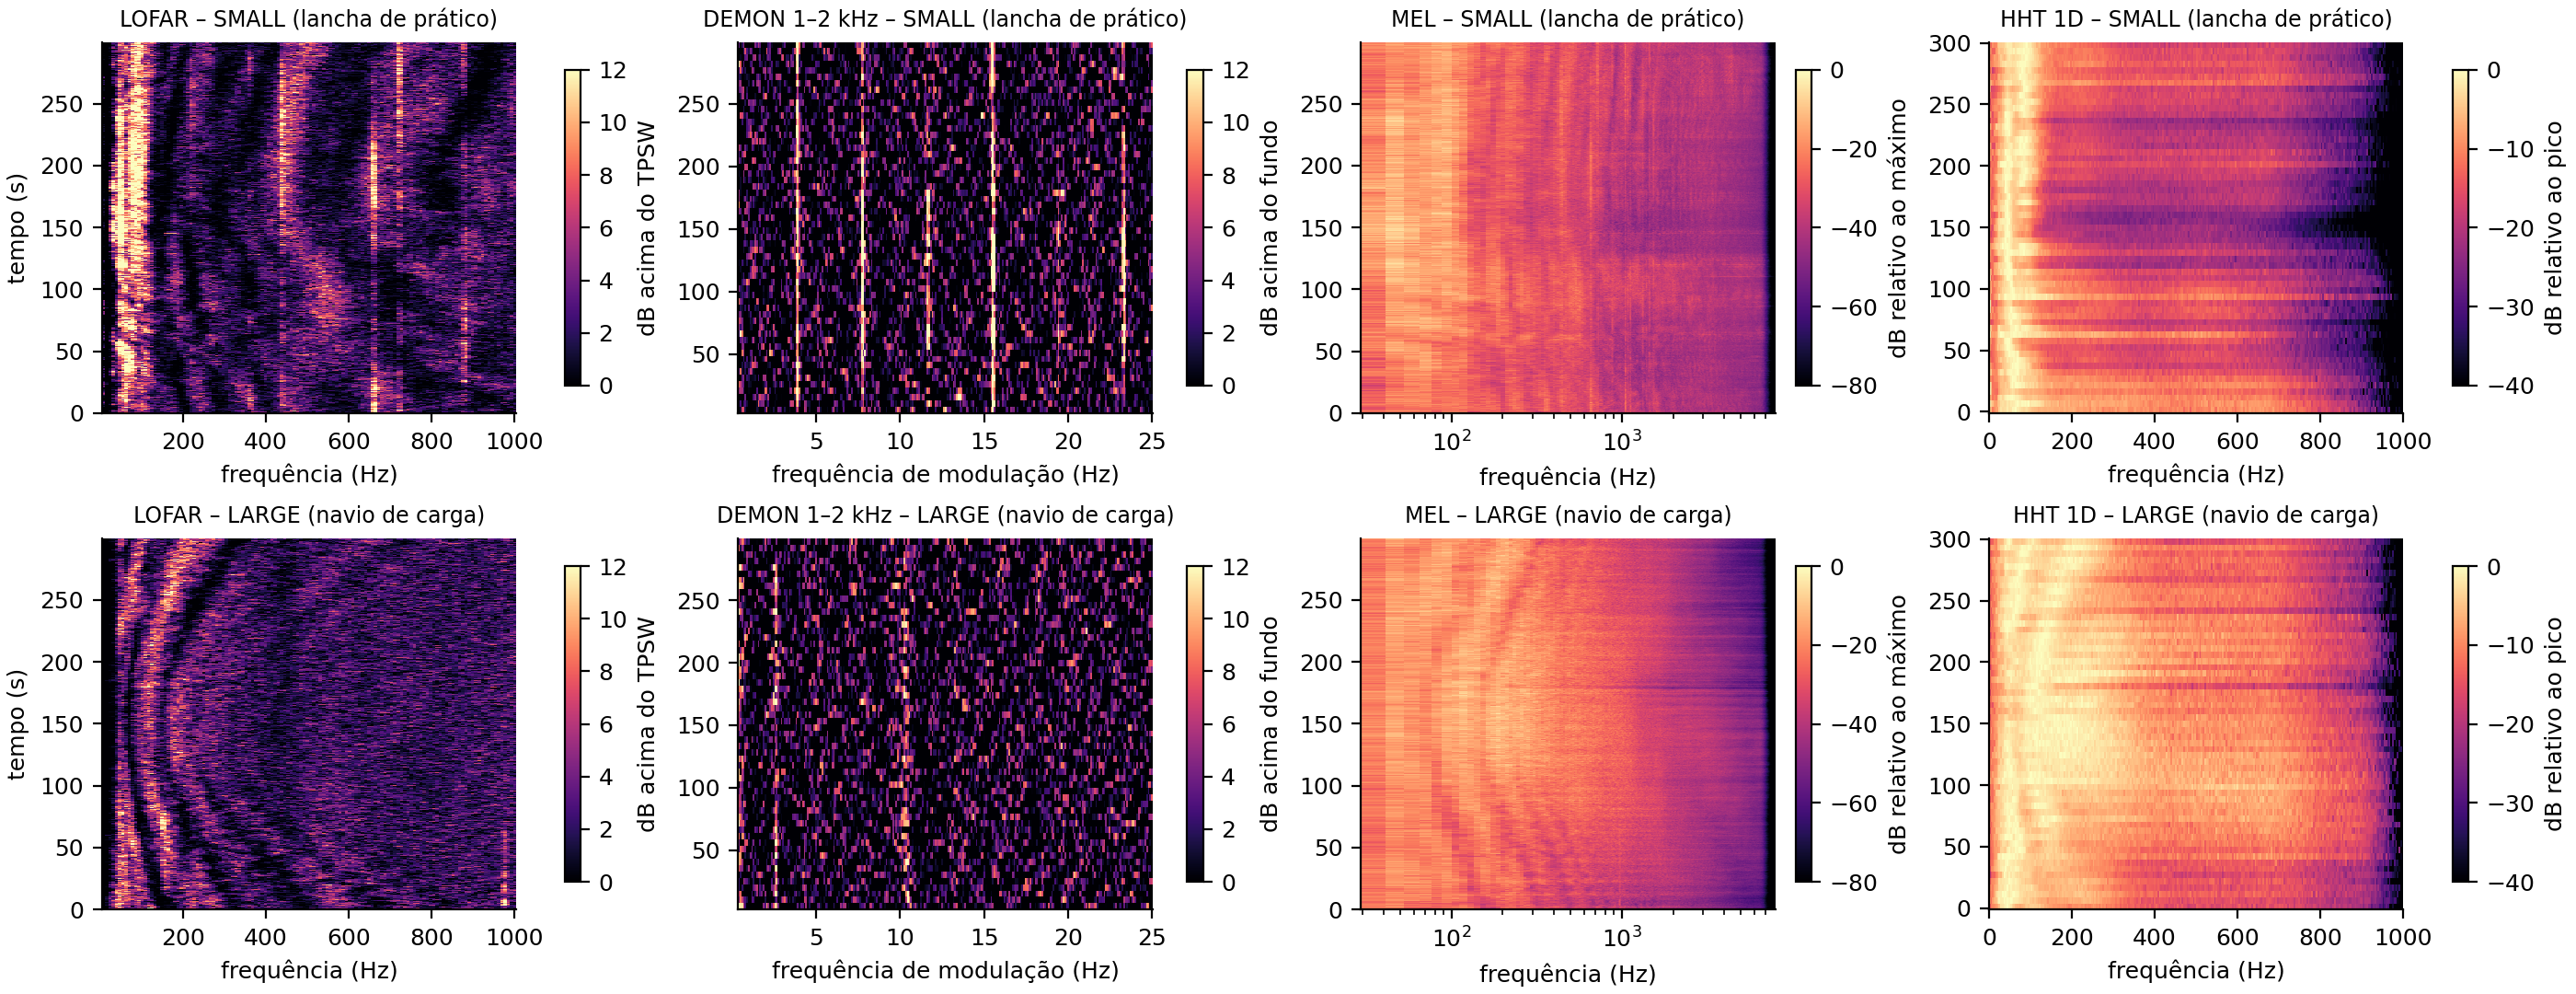
\includegraphics[width=\textwidth]{exemplos_extracoes.png}\\[-1pt]
    \scriptsize
    Lancha PILOT 14 (12 m, subconjunto A) e carga BBC EMSLAND (146 m, subconjunto A). \textbf{LOFAR:} a lancha tem energia em 50--120 Hz e linhas finas até 1 kHz; o carga tem o grave $<$ 100 Hz e o ``U'' do efeito Doppler/distância. \textbf{DEMON:} a lancha mostra uma série de linhas a cada $\sim$3,9 Hz (eixo e harmônicos); o carga, linhas mais graves (2,6 e 10,3 Hz). \textbf{MEL:} o mesmo espectro sem TPSW; o carga concentra a energia abaixo de $\sim$300 Hz. \textbf{HHT 1D:} a lancha tem quase tudo abaixo de 150 Hz; o carga espalha a energia até 1 kHz.
\end{frame}

%===========================================
% SEÇÃO 3 - COMO O MODELO TRATA O SMALL
%===========================================
\section{Como os Modelos Tratam o SMALL}

\begin{frame}
    \centering
    \huge Como os Modelos Tratam o SMALL
\end{frame}

\begin{frame}{Para Onde Vão as SMALL (MLP LOFAR, 4 Classes)}
    \footnotesize
    \begin{columns}[T]
        \begin{column}{0.52\textwidth}
            \centering
            \scriptsize
            \textbf{Split por navio} (navios nunca vistos; \% por linha)\\[2pt]
            \setlength{\tabcolsep}{3pt}
            \begin{tabular}{@{}lcccc@{}}
                \toprule
                Real $\downarrow$ / Prevista $\to$ & SMALL & MEDIUM & LARGE & BG \\
                \midrule
                SMALL & \cahi{48,9} & 22,9 & 23,9 & 4,2 \\
                MEDIUM & \calo{51,0} & 32,3 & 15,3 & 1,4 \\
                LARGE & 20,3 & 10,5 & \cahi{67,7} & 1,6 \\
                BG & 11,3 & 4,3 & 3,3 & \cahi{81,1} \\
                \bottomrule
            \end{tabular}\\[6pt]
            \textbf{Recall por split}\\[2pt]
            \begin{tabular}{@{}lccc@{}}
                \toprule
                Classe & Por gravação & Por navio & Queda \\
                \midrule
                SMALL & 54,0 & 48,9 & $-$5 \\
                MEDIUM & 65,8 & 32,3 & \calo{$-$34} \\
                LARGE & 71,2 & 67,7 & $-$4 \\
                \bottomrule
            \end{tabular}
        \end{column}
        \begin{column}{0.46\textwidth}
            \begin{block}{\small Leitura}
                \scriptsize
                \begin{itemize}
                    \setlength{\itemsep}{2pt}
                    \item O SMALL \textbf{não é decorado}: o recall quase não cai com navios nunca vistos (o MEDIUM cai pela metade).
                    \item Mas fica em $\sim$50\%: os erros se dividem entre \textbf{MEDIUM (23\%)} e \textbf{LARGE (24\%)}.
                    \item \textbf{O MEDIUM ``vira'' SMALL} (51\%): para o modelo, os dois soam iguais.
                    \item 11\% do BACKGROUND é chamado de SMALL: o fundo não está totalmente resolvido.
                \end{itemize}
            \end{block}
        \end{column}
    \end{columns}
\end{frame}

\begin{frame}{O Acerto É Igual nos Três Tipos de SMALL}
    \footnotesize
    \begin{columns}[T]
        \begin{column}{0.50\textwidth}
            \centering
            \scriptsize
            \textbf{MLP LOFAR, split por navio: \% por destino}\\[3pt]
            \tiny\setlength{\tabcolsep}{3pt}
            \begin{tabular}{@{}lrcccc@{}}
                \toprule
                Tipo & Navios & SMALL & MEDIUM & LARGE & BG \\
                \midrule
                Lancha de prático & 15 & 49 & 22 & 24 & 4 \\
                Rebocador & 34 & 45 & 24 & 26 & 5 \\
                Pesca & 22 & 50 & 17 & 30 & 3 \\
                Outros & 16 & 54 & 33 & 12 & 2 \\
                \bottomrule
            \end{tabular}\\[6pt]
            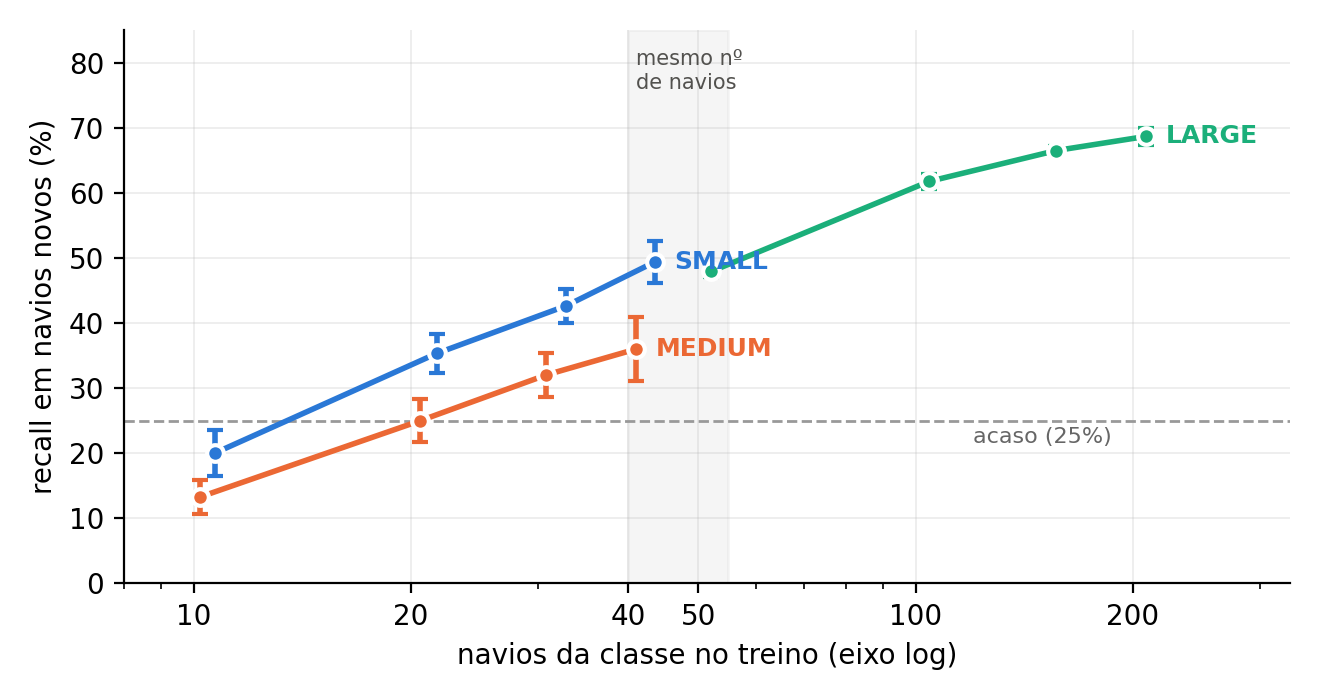
\includegraphics[width=0.92\textwidth]{curva_navios.png}
        \end{column}
        \begin{column}{0.48\textwidth}
            \begin{block}{\small Leitura}
                \scriptsize
                \begin{itemize}
                    \setlength{\itemsep}{2pt}
                    \item Rebocadores e pesca, com muitos navios de poucas gravações, acertam \textbf{tanto quanto as lanchas}: não é só decorar 5 lanchas.
                    \item \textbf{Mas as lanchas sustentam o recall:} com peso igual por navio no treino, o recall de SMALL cai de 49\% para 32\%.
                    \item \textbf{Curva por nº de navios} (NB39, gráfico): o recall de SMALL sobe $\sim$14 pontos a cada vez que o nº de navios dobra (20\% com 11 navios $\to$ 49\% com 44). Com o mesmo nº de navios, SMALL acerta como LARGE.
                    \item Navios gravados uma só vez: 20\% de acerto (CNN do artigo); com mais de 10 gravações, 26\%. Mesmo conhecendo o navio, o SMALL é difícil.
                \end{itemize}
            \end{block}
        \end{column}
    \end{columns}
\end{frame}

%===========================================
% SEÇÃO 4 - LOFAR
%===========================================
\section{O Que o LOFAR Mostra}

\begin{frame}
    \centering
    \huge O Que o LOFAR Mostra
\end{frame}

\begin{frame}{LOFAR Médio por Classe e por Tipo de SMALL}
    \centering
    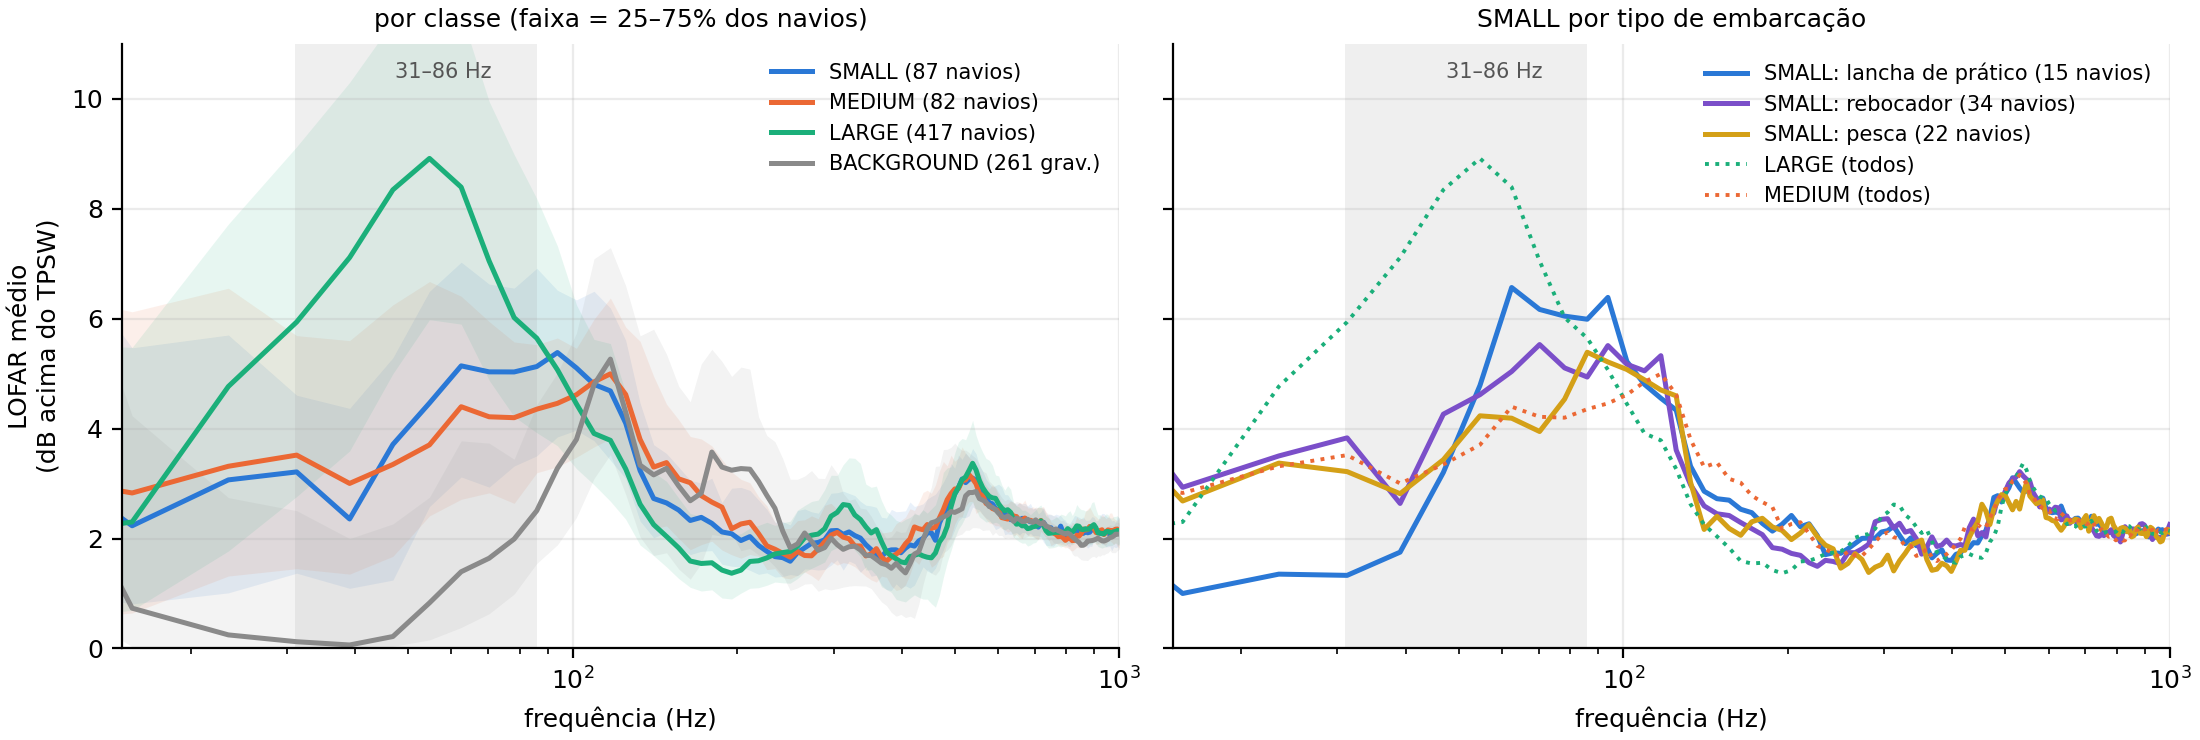
\includegraphics[width=0.93\textwidth]{lofar_classes.png}\\[-1pt]
    \scriptsize
    Mediana entre navios do LOFAR médio de cada gravação (dB acima do TPSW). \textbf{Esquerda:} o LARGE tem a banda de 31--86 Hz (pico em 55 Hz, $\sim$9 dB); \textbf{SMALL e MEDIUM se sobrepõem}, com o máximo em 60--120 Hz e $\sim$5 dB. \textbf{Direita:} os três tipos de SMALL têm o mesmo desenho; a lancha tem menos grave abaixo de 40 Hz. Acima de 250 Hz, todas as classes são iguais.
\end{frame}

\begin{frame}{Onde Fica o Pico Grave de Cada Navio}
    \footnotesize
    \begin{columns}[T]
        \begin{column}{0.60\textwidth}
            \centering
            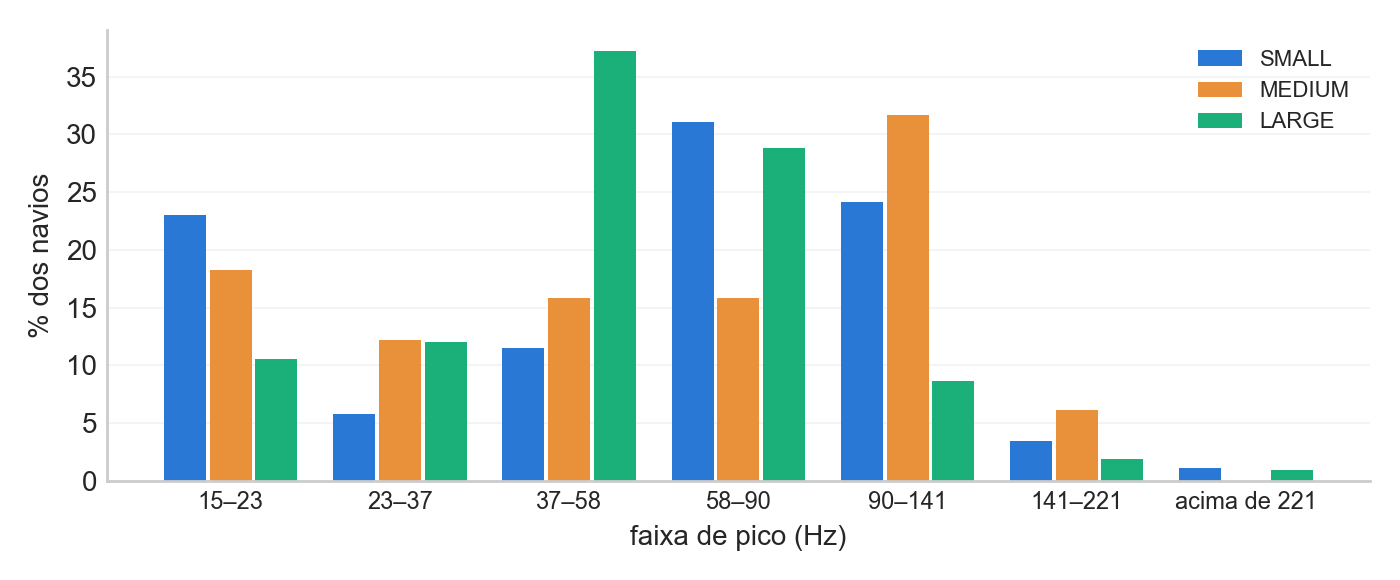
\includegraphics[width=\textwidth]{pico_classes.png}\\
            \scriptsize Faixa do pico de energia no LOFAR (15--250 Hz), um ponto por navio (NB40).
        \end{column}
        \begin{column}{0.38\textwidth}
            \begin{block}{\small Leitura}
                \scriptsize
                \begin{itemize}
                    \setlength{\itemsep}{2pt}
                    \item \textbf{LARGE:} 66\% dos navios com pico em 37--90 Hz.
                    \item \textbf{SMALL:} espalhado; a faixa mais comum é 58--90 Hz (31\%), depois 90--141 Hz (24\%) e 15--23 Hz (23\%).
                    \item \textbf{MEDIUM:} mais comum em 90--141 Hz (32\%).
                    \item \textbf{Nenhuma faixa é ``do SMALL''.} Entre SMALL e MEDIUM, o pico do menor navio é até \textbf{mais grave}: o tamanho não acompanha a frequência abaixo de 100 m.
                    \item Ter o pico em 31--86 Hz: LARGE 72\%, \textbf{SMALL 43\%}, MEDIUM 35\% das gravações.
                \end{itemize}
            \end{block}
        \end{column}
    \end{columns}
\end{frame}

\begin{frame}{SMALL Acertadas e Erradas: o Espectro de Cada Destino}
    \footnotesize
    \begin{columns}[T]
        \begin{column}{0.60\textwidth}
            \centering
            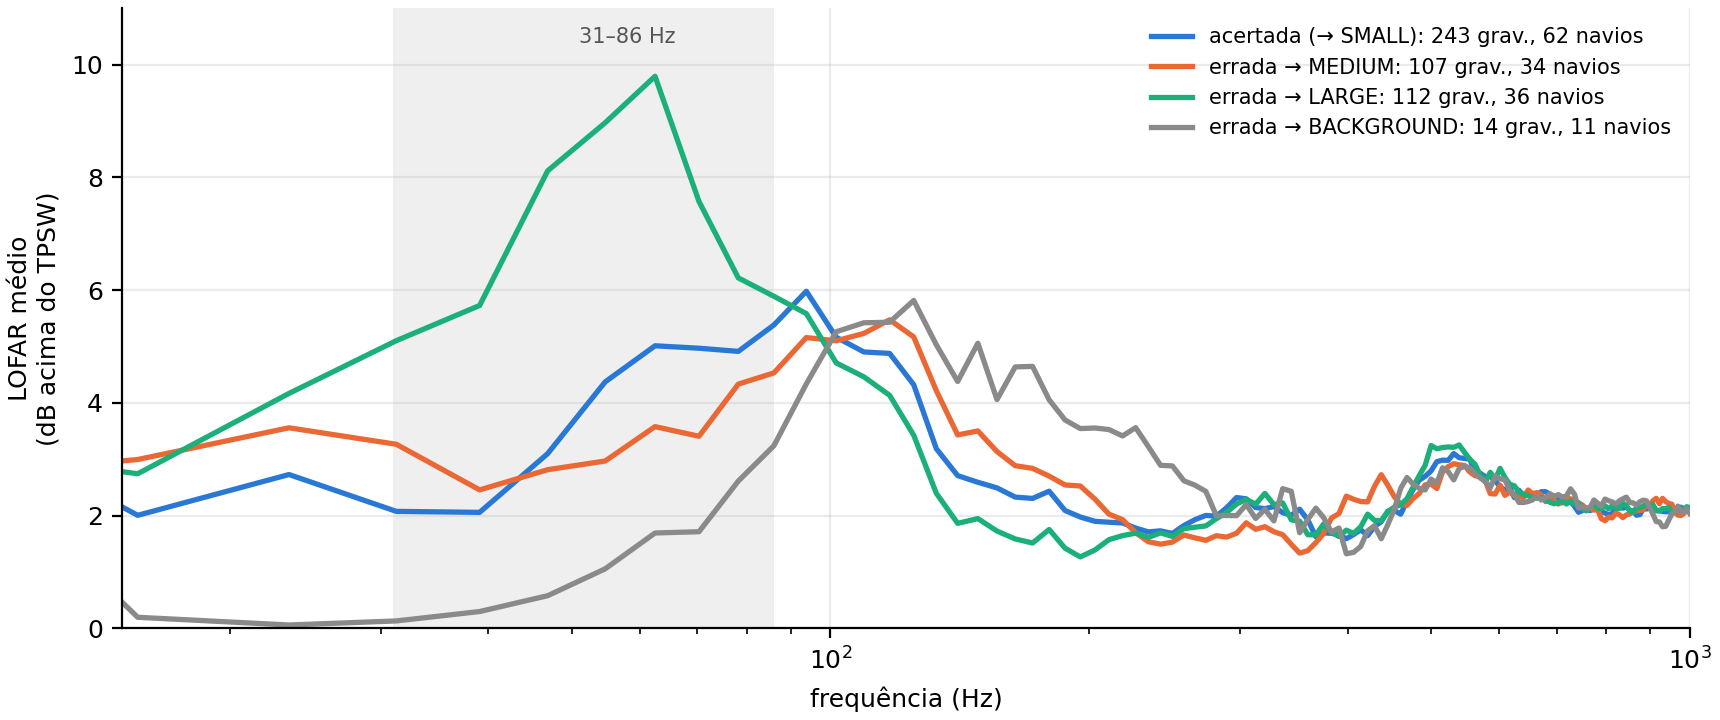
\includegraphics[width=\textwidth]{lofar_destinos.png}\\
            \scriptsize Destino = classe mais prevista nas 5 avaliações (MLP LOFAR 4 classes, split por navio); mediana entre navios.
        \end{column}
        \begin{column}{0.38\textwidth}
            \begin{block}{\small Leitura (confirma o NB35)}
                \scriptsize
                \begin{itemize}
                    \setlength{\itemsep}{2pt}
                    \item \textbf{$\to$ LARGE:} têm a banda de 31--86 Hz no nível das LARGE (pico de $\sim$10 dB). No NB35, AUC 0,85, confirmado fora da amostra (a banda foi achada só com navios LARGE).
                    \item \textbf{Acertadas:} máximo em $\sim$95 Hz, acima da banda das LARGE.
                    \item \textbf{$\to$ MEDIUM:} menos energia em 40--90 Hz e o máximo deslocado para $\sim$120 Hz; no NB35, diferenças só minúsculas ($\sim$0,1 dB) acima de 1 kHz.
                    \item \textbf{$\to$ BACKGROUND} (poucas): quase sem grave; o navio mal aparece.
                \end{itemize}
            \end{block}
        \end{column}
    \end{columns}
\end{frame}

\begin{frame}{A Banda de 31--86 Hz É Pista do Modelo, Não do Tamanho}
    \footnotesize
    \begin{columns}[T]
        \begin{column}{0.48\textwidth}
            \centering
            \scriptsize
            \textbf{\% das gravações chamadas de LARGE (CNN LOFAR do artigo)}\\[3pt]
            \begin{tabular}{@{}lcc@{}}
                \toprule
                Classe real & Sem a banda & Com a banda \\
                \midrule
                SMALL & 11\% & \calo{37\%} \\
                MEDIUM & 6\% & 23\% \\
                LARGE & 39\% & \cahi{83\%} \\
                \bottomrule
            \end{tabular}\\[6pt]
            \textbf{Quem tem a banda (pico em 31--86 Hz)}\\[3pt]
            \begin{tabular}{@{}lc@{}}
                \toprule
                Classe & \% das gravações \\
                \midrule
                SMALL & 43\% \\
                MEDIUM & 35\% \\
                LARGE & 72\% \\
                \bottomrule
            \end{tabular}
        \end{column}
        \begin{column}{0.50\textwidth}
            \begin{block}{\small Leitura}
                \scriptsize
                \begin{itemize}
                    \setlength{\itemsep}{2pt}
                    \item Em qualquer classe, \textbf{ter a banda aumenta a chance de a gravação ser chamada de LARGE}. Não é regra: 63\% das SMALL com a banda continuam fora de LARGE.
                    \item Mas a banda é \textbf{fraca como pista de tamanho}: das gravações com a banda, só 55\% são LARGE.
                    \item É banda larga ($\sim$55 Hz), não raias: com faixas de 1 Hz (lofar1hz), o número e a energia das raias estreitas não diferem entre os grupos.
                    \item \textbf{O modelo reconhece o SMALL pela falta da banda}, e erra quando ela aparece.
                \end{itemize}
            \end{block}
        \end{column}
    \end{columns}
\end{frame}

\begin{frame}{Ao Longo da Passagem: o SMALL Mal Muda}
    \footnotesize
    \begin{columns}[T]
        \begin{column}{0.56\textwidth}
            \centering
            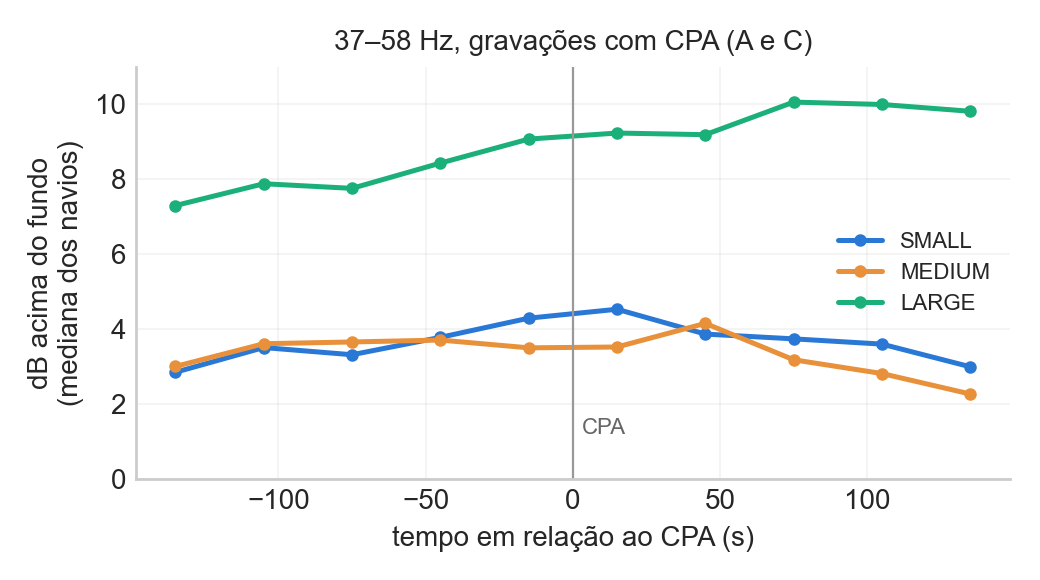
\includegraphics[width=\textwidth]{energia_passagem.png}\\
            \scriptsize LOFAR em 37--58 Hz em 10 fatias de 30 s em torno do CPA (subconjuntos A e C), mediana dos navios (NB40).
        \end{column}
        \begin{column}{0.42\textwidth}
            \begin{block}{\small Leitura}
                \scriptsize
                \begin{itemize}
                    \setlength{\itemsep}{2pt}
                    \item \textbf{LARGE:} o grave sobe de 7,3 para 9,8 dB e continua alto depois do CPA.
                    \item \textbf{SMALL e MEDIUM:} só um ``morrinho'' de 1 a 1,5 dB perto do CPA.
                    \item SMALL $\times$ MEDIUM: \textbf{0 diferenças em 140 testes} (14 faixas $\times$ 10 fatias). SMALL $\times$ LARGE: 100/140.
                    \item O que separa os navios $<$ 100 m dos LARGE: mais energia em \textbf{90--221 Hz} e menos abaixo de 90 Hz, em todos os momentos da passagem.
                \end{itemize}
            \end{block}
        \end{column}
    \end{columns}
\end{frame}

\begin{frame}{Lanchas de Prático: Por Que Erra Mesmo Conhecendo a Lancha}
    \footnotesize
    \begin{columns}[T]
        \begin{column}{0.58\textwidth}
            \centering
            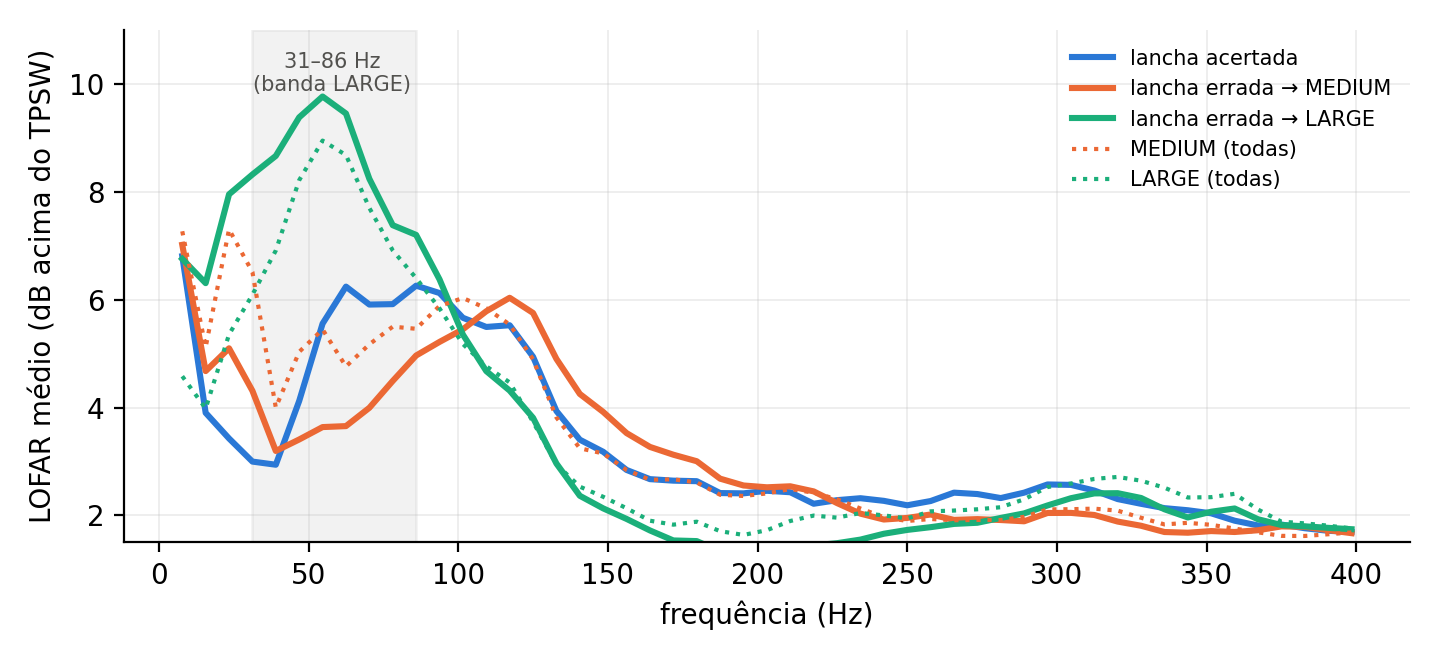
\includegraphics[width=\textwidth]{lancha_espectro.png}\\
            \scriptsize Split por gravação (a lancha está no treino); errada = acertada em menos da metade das 5 avaliações (NB39, seção 9).
        \end{column}
        \begin{column}{0.40\textwidth}
            \begin{block}{\small Leitura}
                \scriptsize
                \begin{itemize}
                    \setlength{\itemsep}{2pt}
                    \item $\sim$45\% das gravações erradas \textbf{mesmo com a lancha no treino}; metade vai para MEDIUM, metade para LARGE.
                    \item \textbf{$\to$ LARGE:} grave de 31--86 Hz em 8,6 dB, mais que a média das LARGE (7,5 dB). Só há um navio por gravação.
                    \item \textbf{Na mesma lancha}, as erradas têm menos energia de 250 Hz a 8 kHz (AUC 0,29) e sinal acima do fundo 3 dB menor.
                    \item Vento e duração não importam; B (perto, sem CPA) é o pior (59\% erradas).
                    \item Hipóteses não testáveis no IARA: outro regime da lancha ou grave do local.
                \end{itemize}
            \end{block}
        \end{column}
    \end{columns}
\end{frame}

%===========================================
% SEÇÃO 5 - DEMON
%===========================================
\section{O Que o DEMON Mostra}

\begin{frame}
    \centering
    \huge O Que o DEMON Mostra
\end{frame}

\begin{frame}{DEMON Médio: as Linhas de Cada Navio Se Apagam na Média}
    \centering
    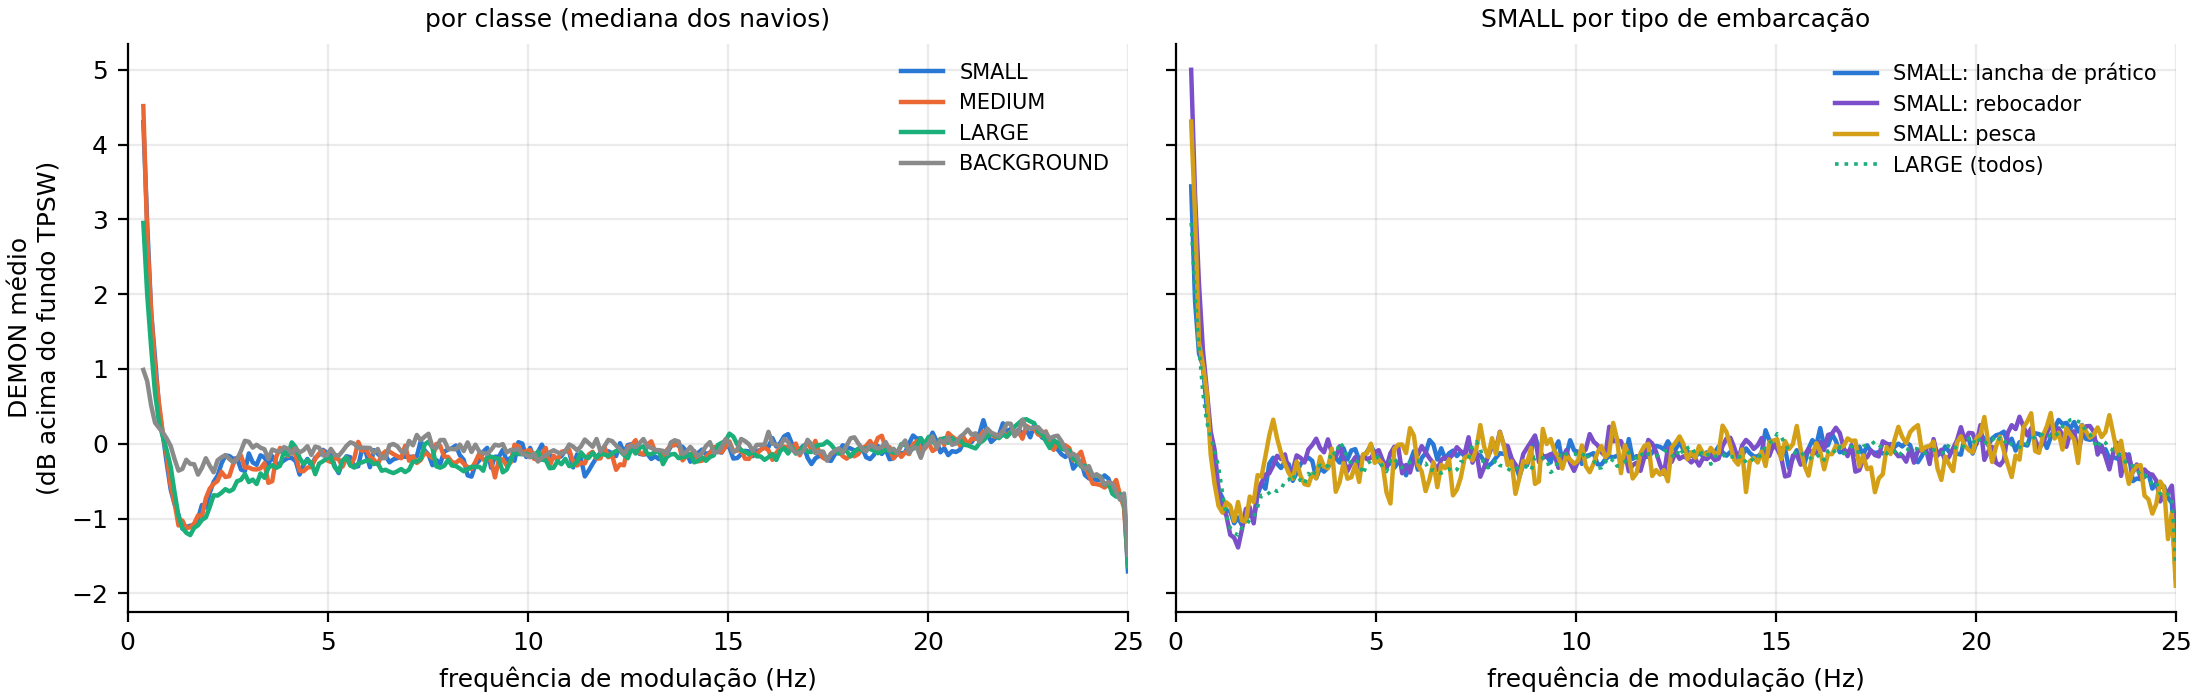
\includegraphics[width=0.93\textwidth]{demon_classes.png}\\[-1pt]
    \scriptsize
    Mediana entre navios do DEMON médio de cada gravação (dB acima do fundo TPSW). Todas as curvas ficam perto de 0 dB: cada navio tem as suas linhas em frequências próprias (exemplo do slide 14), e na média elas se espalham e somem. Faixa a faixa, SMALL $\times$ MEDIUM: \textbf{0 faixas diferentes} (de 253). A informação do DEMON está no \textbf{pico de cada gravação} (próximo slide).
\end{frame}

\begin{frame}{DEMON: a Linha Mais Forte de Cada Navio}
    \footnotesize
    \centering
    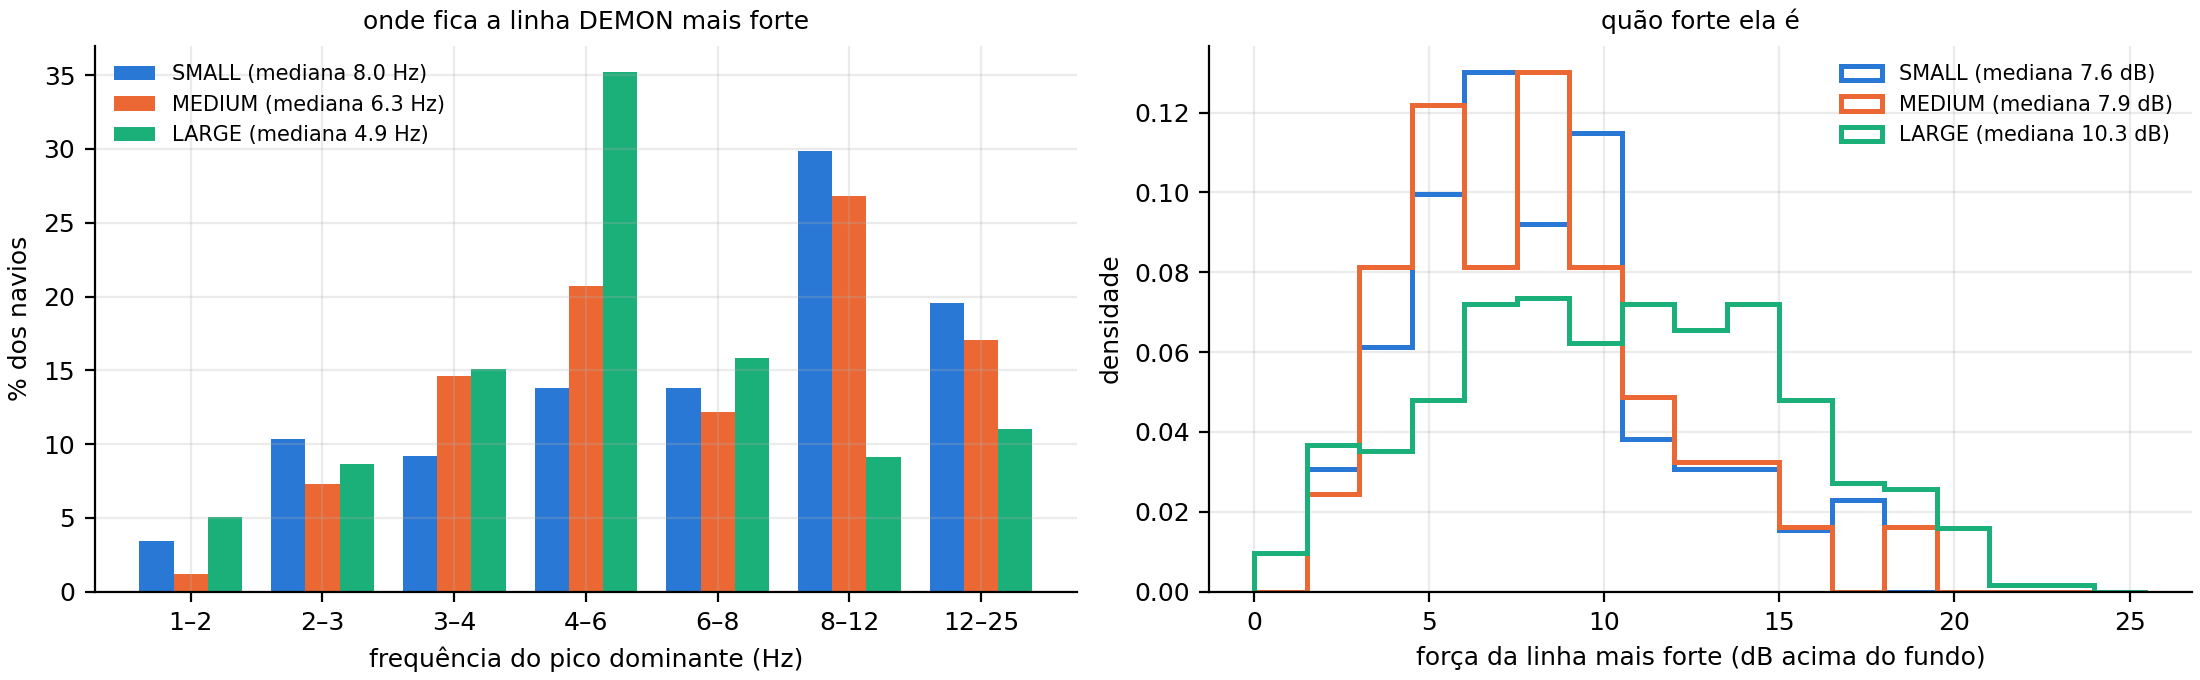
\includegraphics[width=0.86\textwidth]{demon_pico.png}\\[2pt]
    \begin{columns}[T]
        \begin{column}{0.49\textwidth}
            \scriptsize
            \begin{itemize}
                \setlength{\itemsep}{1pt}
                \item Pico dominante a partir de 1 Hz, mediana por navio. \textbf{LARGE:} mais grave (4,9 Hz) e mais forte (10,3 dB).
                \item \textbf{SMALL (8,0 Hz; 7,6 dB) e MEDIUM (6,3 Hz; 7,9 dB):} distribuições parecidas, linha mais rasa.
            \end{itemize}
        \end{column}
        \begin{column}{0.49\textwidth}
            \scriptsize
            \begin{itemize}
                \setlength{\itemsep}{1pt}
                \item NB36 (estimativa da fundamental): SMALL 6,3, MEDIUM 6,4, LARGE 2,4 Hz; ela só cai acima de $\sim$200 m (4--5 Hz de 25 a 200 m).
                \item Pico forte ($\geq$ 10 dB): LARGE 49\%, SMALL 28\%, MEDIUM 24\%. É pista de LARGE, como a banda do LOFAR.
            \end{itemize}
        \end{column}
    \end{columns}
\end{frame}

\begin{frame}{DEMON nas Lanchas e Como Classificador}
    \footnotesize
    \begin{columns}[T]
        \begin{column}{0.56\textwidth}
            \centering
            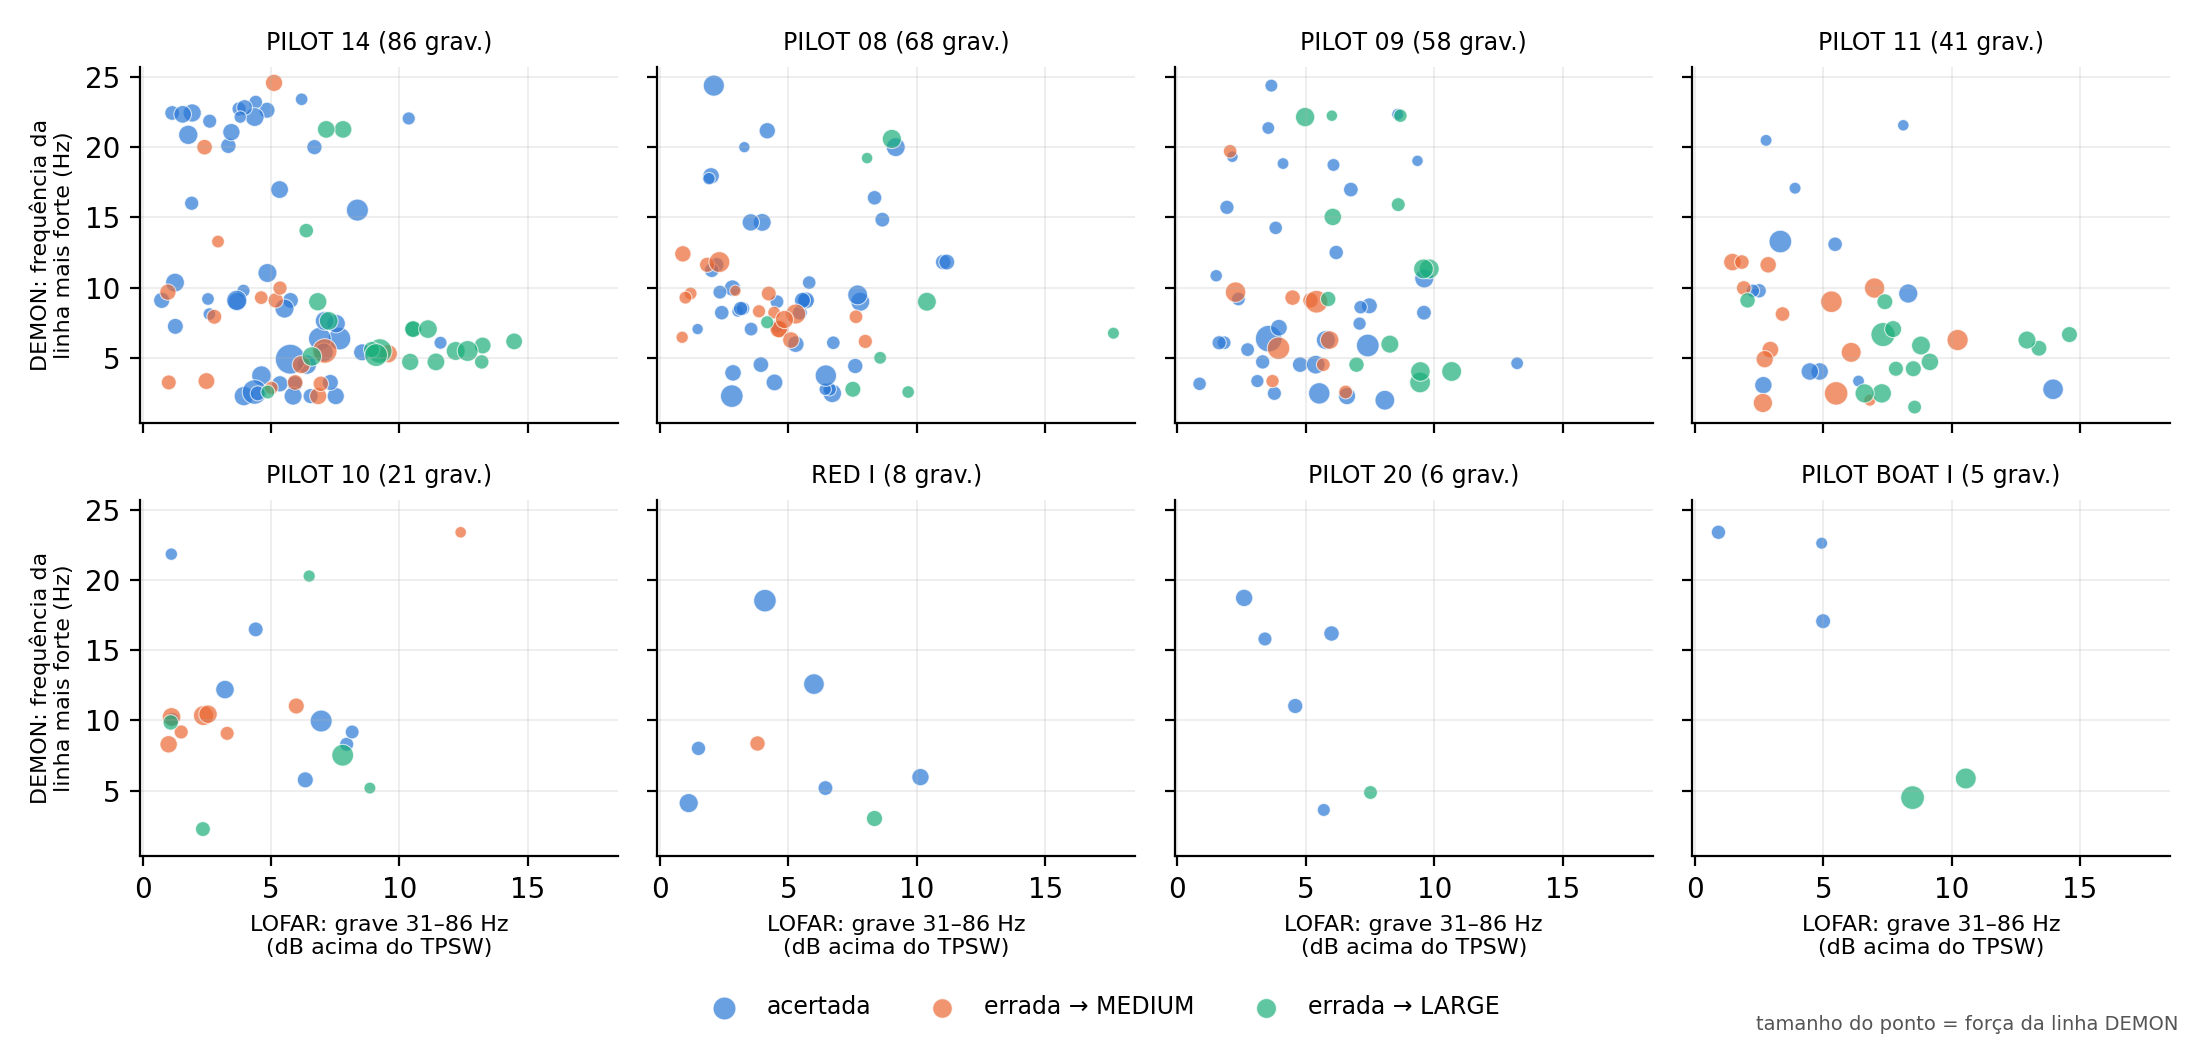
\includegraphics[width=\textwidth]{lanchas_lofar_demon.png}\\
            \scriptsize Cada ponto é uma gravação de uma lancha: x = grave LOFAR, y = frequência da linha DEMON, tamanho = força.
        \end{column}
        \begin{column}{0.42\textwidth}
            \begin{block}{\small Dentro da mesma lancha (AUC)}
                \scriptsize
                \begin{tabular}{@{}lccc@{}}
                    \toprule
                    & LOFAR & \multicolumn{2}{c}{DEMON} \\
                    & 31--86 Hz & força & freq. \\
                    \midrule
                    $\to$L $\times$ acertada & \cahi{0,80} & 0,57 & 0,39 \\
                    $\to$L $\times$ $\to$M & \cahi{0,87} & 0,52 & 0,47 \\
                    $\to$M $\times$ acertada & 0,44 & 0,51 & 0,43 \\
                    \bottomrule
                \end{tabular}
            \end{block}
            \begin{block}{\small Leitura}
                \scriptsize
                \begin{itemize}
                    \setlength{\itemsep}{1pt}
                    \item Na mesma lancha, quem explica o erro $\to$ LARGE é o \textbf{grave do LOFAR}; o DEMON quase não acrescenta.
                    \item \textbf{MLP só com DEMON:} recall de SMALL $\sim$28\% (acaso 25\%).
                    \item \textbf{SMALL $\times$ MEDIUM só com DEMON:} AUC 0,48 (acaso).
                \end{itemize}
            \end{block}
        \end{column}
    \end{columns}
\end{frame}

%===========================================
% SEÇÃO 6 - MEL E HHT
%===========================================
\section{O Que o MEL e o HHT Mostram}

\begin{frame}
    \centering
    \huge O Que o MEL e o HHT Mostram
\end{frame}

\begin{frame}{MEL e HHT por Classe}
    \centering
    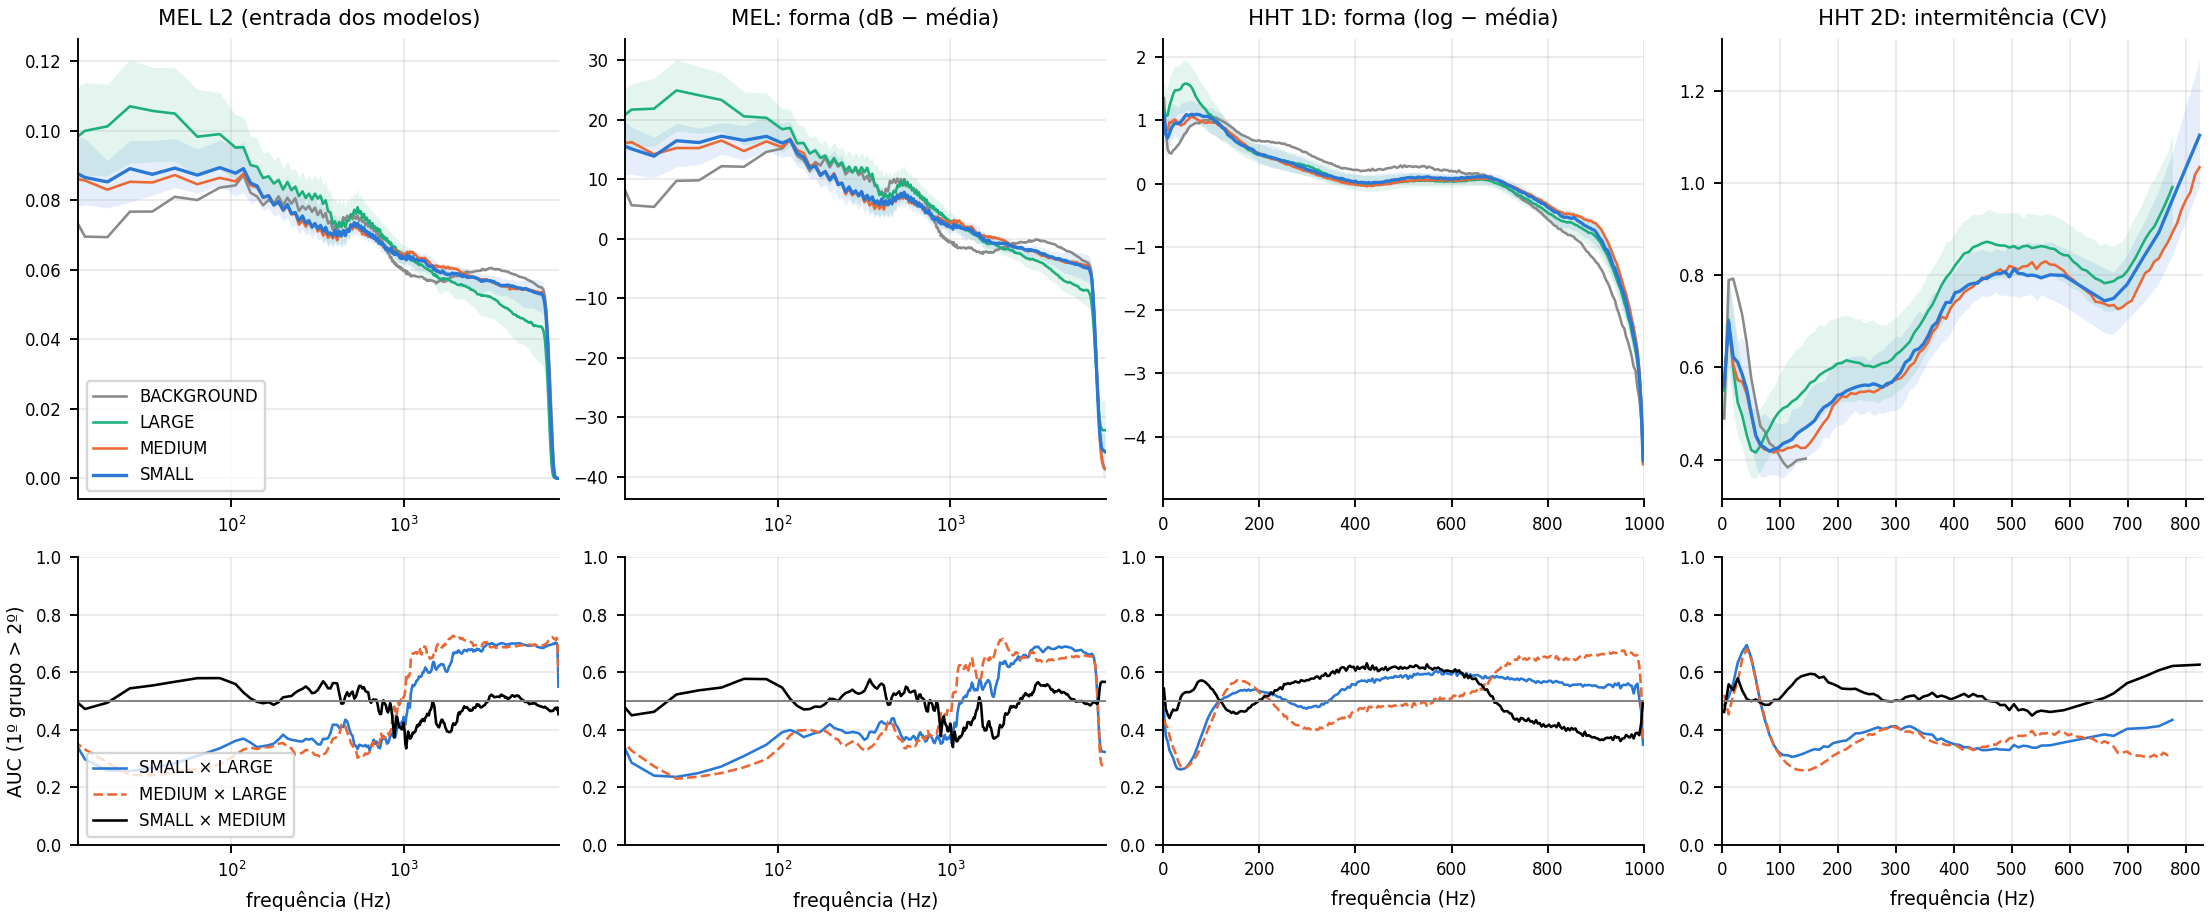
\includegraphics[width=\textwidth]{mel_hht_classes.png}\\[-1pt]
    \scriptsize
    \textbf{Em cima:} mediana entre navios (faixa = 25--75\% em SMALL e LARGE). \textbf{Embaixo:} AUC faixa a faixa (0,5 = sem diferença). A curva azul (SMALL $\times$ LARGE) e a laranja tracejada (MEDIUM $\times$ LARGE) andam juntas; a preta (SMALL $\times$ MEDIUM) fica perto de 0,5.
\end{frame}

\begin{frame}{MEL e HHT: Existe Algo que Só o SMALL Tem?}
    \footnotesize
    \begin{columns}[T]
        \begin{column}{0.52\textwidth}
            \scriptsize
            Faixas com q $<$ 0,05, \textbf{dentro} de cada subconjunto (A / C / D):\\[3pt]
            \tiny
            \setlength{\tabcolsep}{2.5pt}
            \begin{tabular}{@{}lccc@{}}
                \toprule
                & S $\times$ M & S $\times$ L & M $\times$ L \\
                \midrule
                MEL L2 (256) & 0 / 0 / 0 & 215 / 241 / \textbf{0} & 236 / 234 / 206 \\
                MEL forma (256) & 0 / 0 / 0 & 187 / 206 / \textbf{0} & 231 / 234 / 19 \\
                HHT 1D forma (256) & 0 / 0 / 0 & 86 / 61 / \textbf{0} & 103 / 94 / 82 \\
                HHT 2D intermit. & 0 / 0 / 0 & 74 / 10 / 96 & 111 / 40 / 62 \\
                \bottomrule
            \end{tabular}\\[4pt]
            \tiny S = SMALL, M = MEDIUM, L = LARGE. AUC S$\times$L contra AUC M$\times$L, faixa a faixa: correlação de 0,96 (MEL L2), 0,92 (MEL forma), 0,91 (intermitência) e 0,69 (HHT 1D); diferença máxima de 0,15.
        \end{column}
        \begin{column}{0.45\textwidth}
            \begin{block}{\small Leitura}
                \scriptsize
                \begin{itemize}
                    \setlength{\itemsep}{2pt}
                    \item \textbf{SMALL $\times$ MEDIUM: 0 faixas} em todas as representações, dentro de todos os subconjuntos.
                    \item \textbf{SMALL $\times$ LARGE} repete MEDIUM $\times$ LARGE: o LARGE tem mais grave ($<$ 1 kHz); o ``mais agudo'' do SMALL é só \textbf{efeito da normalização}.
                    \item \textbf{Intermitência:} maior no LARGE fora do pico grave; é quase toda \textbf{energia relativa} ($\rho$ = $-$0,92), pois o HHT 2D divide pelo pico.
                    \item \textbf{Subconjunto D} (sem CPA, 250--500 m): o MEL não separa SMALL de LARGE, mas separa MEDIUM de LARGE.
                \end{itemize}
            \end{block}
        \end{column}
    \end{columns}
\end{frame}

\begin{frame}{HHT: a Única Pista SMALL $\times$ MEDIUM (NB37 e NB38)}
    \footnotesize
    \begin{columns}[T]
        \begin{column}{0.49\textwidth}
            \begin{block}{\small O que apareceu}
                \scriptsize
                \begin{itemize}
                    \setlength{\itemsep}{2pt}
                    \item Na comparação dos tipos, \textbf{rebocador (SMALL) $\times$ apoio offshore (MEDIUM)}: o rebocador parece mais ``intermitente'' em 100--200 Hz (AUC 0,28, q 0,007) e 730--830 Hz.
                    \item Mesmo sentido nos 4 subconjuntos; em metades de navios, mesmo sentido em 95\%, mas significativo em só 46\%.
                    \item Em \textbf{SMALL $\times$ MEDIUM} (classes inteiras), mais fraco: 720--830 Hz, AUC 0,39 (p 0,011); 0 faixas com FDR.
                \end{itemize}
            \end{block}
        \end{column}
        \begin{column}{0.49\textwidth}
            \begin{block}{\small O que isso significa}
                \scriptsize
                \begin{itemize}
                    \setlength{\itemsep}{2pt}
                    \item Não é ``oscila mais no tempo'': é que o apoio offshore tem \textbf{relativamente mais energia em 100--200 Hz} (AUC 0,71); o resto da intermitência é fraco (AUC 0,37, p 0,045).
                    \item É uma pista de \textbf{tipo} (rebocador $\times$ supply), não de tamanho, e está no sentido ``o MEDIUM tem mais''.
                    \item \textbf{Como classificador} (NB38, CV por navio): SMALL $\times$ MEDIUM sobe de AUC 0,54 (LOFAR) para 0,59 com a intermitência. Consistente, mas perto do acaso.
                \end{itemize}
            \end{block}
        \end{column}
    \end{columns}
\end{frame}

%===========================================
% SEÇÃO 7 - O QUE NÃO FUNCIONOU
%===========================================
\section{O Que Já Testamos para o SMALL}

\begin{frame}
    \centering
    \huge O Que Já Testamos para o SMALL
\end{frame}

\begin{frame}{SMALL $\times$ MEDIUM e o Experimento mix\_small\_medium}
    \footnotesize
    \begin{columns}[T]
        \begin{column}{0.50\textwidth}
            \centering
            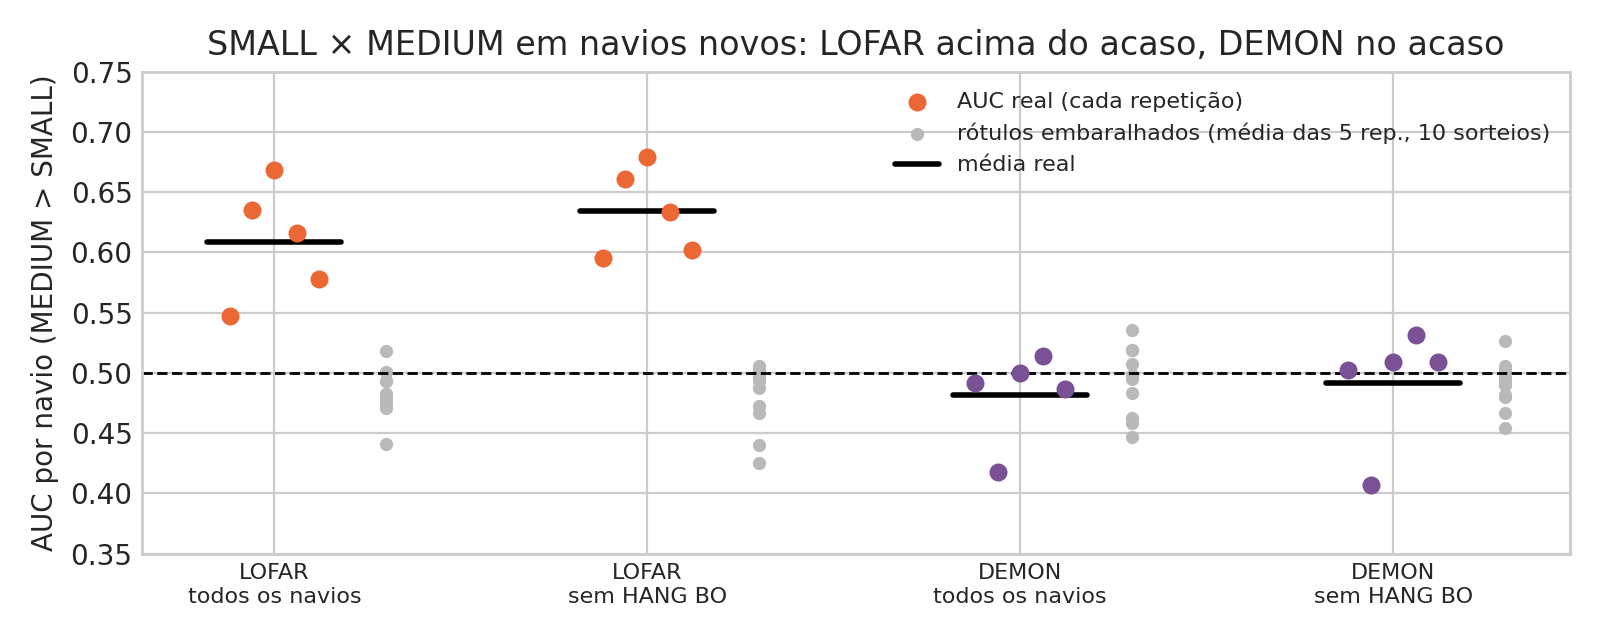
\includegraphics[width=\textwidth]{small_vs_medium_auc.png}\\
            \scriptsize MLP só com SMALL e MEDIUM, split por navio; AUC por navio contra rótulos embaralhados entre navios (NB39, seção 11).
        \end{column}
        \begin{column}{0.48\textwidth}
            \begin{block}{\small SMALL $\times$ MEDIUM dedicado}
                \scriptsize
                \begin{itemize}
                    \setlength{\itemsep}{1pt}
                    \item \textbf{LOFAR:} AUC 0,61 (acaso até 0,52); acerto balanceado só 55,6\%.
                    \item \textbf{DEMON:} AUC 0,48 (acaso).
                    \item Não acompanha o comprimento (Spearman 0,15 em SMALL) nem a fronteira de 50 m. O sinal mais provável é o \textbf{tipo}.
                \end{itemize}
            \end{block}
            \begin{block}{\small mix\_small\_medium (SMALL + MEDIUM numa classe)}
                \scriptsize
                \begin{itemize}
                    \setlength{\itemsep}{1pt}
                    \item MIX\_SMALL\_MEDIUM: recall 76\% em navios nunca vistos.
                    \item A parte SMALL acerta 72\% (MEDIUM 81\%); quando erra, vai para \textbf{LARGE} (24\%): as lanchas com grave forte.
                    \item Pesca 68\%, lancha 71\%, rebocador 71\%.
                \end{itemize}
            \end{block}
        \end{column}
    \end{columns}
\end{frame}

\begin{frame}{Data Augmentation: Por Que Tentamos}
    \footnotesize
    \begin{columns}[T]
        \begin{column}{0.53\textwidth}
            \begin{block}{\small O que vimos antes de tentar}
                \scriptsize
                \begin{itemize}
                    \setlength{\itemsep}{2pt}
                    \item \textbf{Faltam navios:} o SMALL equivale a $\sim$12 navios; com o mesmo nº de navios, SMALL e LARGE acertam parecido, e a curva ``acerto $\times$ nº de navios'' ainda subia.
                    \item \textbf{O modelo decora o navio:} MEDIUM com muitas gravações acerta 77\% quando o navio está no treino e 32\% quando não está.
                    \item \textbf{Poucos navios dominam:} 5 lanchas de prático são 59\% do SMALL.
                    \item \textbf{O ambiente pesa na decisão:} uma SMALL gravada num ``ambiente de MEDIUM'' acerta 38\% contra 58\%.
                    \item \textbf{Mar agitado:} o acerto de LARGE cai $\sim$10 pontos.
                \end{itemize}
            \end{block}
        \end{column}
        \begin{column}{0.45\textwidth}
            \begin{block}{\small A ideia}
                \scriptsize
                Se não há mais navios, \textbf{criar variações artificiais} das gravações que existem, imitando o que um navio novo mudaria: rotação, raias, mistura de navios, outro mar.\\[3pt]
                Assim o modelo aprenderia a classe, e não o navio ou o ambiente da gravação.
            \end{block}
            \begin{alertblock}{\small Como foi avaliado}
                \scriptsize
                Split por navio, mesmos folds e modelos da base; o \textbf{teste é sempre o áudio original}. Ganho real (definido antes): +1,5 ponto, p $<$ 0,05 (5x2cv) e melhora em 8 de 10 folds. Controle: cópia idêntica (só repetir os dados).
            \end{alertblock}
        \end{column}
    \end{columns}
\end{frame}

\begin{frame}{Data Augmentation: O Que Foi Tentado}
    \scriptsize
    \centering
    \setlength{\tabcolsep}{4pt}
    \begin{tabularx}{\textwidth}{@{}l>{\raggedright\arraybackslash}X>{\raggedright\arraybackslash}X@{}}
        \toprule
        Variante & O que faz & Problema que ataca \\
        \midrule
        navio & Peso igual por navio (não cria dados) & Domínio das lanchas e das HANG BO \\
        stretch & Estica a frequência em 0,92--1,08 & Outra rotação: as raias mudam de lugar \\
        mask & Apaga 2 faixas de até $\sim$375 Hz & Depender de uma raia de um navio \\
        mixnavio & Mistura 2 navios da mesma classe & ``Navios virtuais'' (faltam navios) \\
        ruído & Ruído gaussiano no LOFAR padronizado & Outra condição de gravação (simplificado) \\
        bg & Soma ao \textbf{áudio} um BACKGROUND real (0--20 dB abaixo) & O mesmo navio em outro mar/ambiente \\
        navio+stretch+mask & As três juntas & Combinação das anteriores \\
        mar agitado & Só LARGE: fundo de mar $\geq$ 4 (controle: calmo) & Queda do LARGE com mar agitado \\
        \bottomrule
    \end{tabularx}\\[3pt]
    \begin{block}{\small Onde foi testado}
        \scriptsize
        MLP, RF, SVM e BiGRU no LOFAR; MLP no DEMON (mar agitado). A CNN do artigo não foi rodada ($\sim$60 h por variante). O LOFAR dos modelos não foi alterado (misturas em pastas próprias). NB39, NB41 e NB42.
    \end{block}
\end{frame}

\begin{frame}{Data Augmentation e Outros Testes: Nada Ajudou o SMALL}
    \scriptsize
    \centering
    \setlength{\tabcolsep}{4pt}
    \begin{tabularx}{0.97\textwidth}{@{}>{\raggedright\arraybackslash}p{3.9cm}>{\raggedright\arraybackslash}X@{}}
        \toprule
        Teste & O que aconteceu com o SMALL \\
        \midrule
        7 augmentations no LOFAR (stretch, mask, mixnavio, ruído, mar real\ldots) em MLP, RF, SVM e BiGRU & Nenhum ganho acima do controle ``cópia idêntica''. Quando o recall de MEDIUM sobe, o de SMALL cai (navio + stretch + mask: SMALL 14\%; SVM com mixnavio: SMALL 20\%). \\
        Peso igual por navio & SMALL cai de 49\% para 32\%: o recall depende das lanchas muito gravadas. \\
        Mistura com mar agitado/calmo nos LARGE (LOFAR, DEMON, SVM) & Sem efeito significativo; as cópias de LARGE com ruído passam a parecer navio $<$ 100 m. \\
        Intermitência do HHT (NB38) & SMALL $\times$ MEDIUM de AUC 0,54 para 0,59: ganho consistente, mas perto do acaso; na prática é energia relativa em 100--200 Hz. \\
        ``Assinatura de ambiente'' (8--23 kHz, trecho mais silencioso) & Quase não indica a classe (AUC 0,51--0,58), mas mexe na decisão: SMALL com ambiente parecido com o de MEDIUM acerta 38\% contra 58\%. \\
        DEMON em 5 bandas, raias de 1 Hz, MEL, HHT & Nenhuma faixa separa SMALL de MEDIUM (nem rebocador de supply) dentro dos subconjuntos. \\
        \bottomrule
    \end{tabularx}
\end{frame}

%===========================================
% SEÇÃO 8 - CONCLUSÕES
%===========================================
\section{Conclusões e Próximos Passos}

\begin{frame}
    \centering
    \huge Conclusões e Próximos Passos
\end{frame}

\begin{frame}{Conclusões}
    \scriptsize
    \begin{enumerate}
        \setlength{\itemsep}{2pt}
        \item \textbf{A classe SMALL do IARA é estreita:} $\sim$12 navios efetivos, dominada por 5 lanchas de prático, e formada por três tipos que só existem nela.
        \item \textbf{O modelo generaliza o SMALL para navios novos em $\sim$50\%}, igual nos três tipos. Isso pode ser ``som desses tipos'' e não ``som de barco pequeno'': o IARA não separa as duas coisas.
        \item \textbf{Não achamos assinatura positiva de SMALL} em nenhuma das extrações:
        \begin{itemize}\scriptsize
            \item LOFAR: o máximo em 60--120 Hz é comum a SMALL e MEDIUM;
            \item DEMON: linha mais rasa e mais aguda que a do LARGE, igual ao MEDIUM;
            \item MEL e HHT: SMALL $\times$ LARGE repete MEDIUM $\times$ LARGE; a ``intermitência'' do HHT é energia relativa e separa tipo (rebocador $\times$ supply), não tamanho.
        \end{itemize}
        \item \textbf{O SMALL é reconhecido pela ausência das pistas do LARGE}; por isso erra para LARGE quando o grave de 31--86 Hz aparece (lanchas, inclusive dentro da mesma lancha), e para BACKGROUND quando o barco mal aparece.
        \item \textbf{SMALL e MEDIUM são acusticamente iguais} em todas as representações e medidas testadas; juntos (navio $<$ 100 m), generalizam bem (76\%).
        \item \textbf{Cuidado com o ``barco que se destaca pouco'':} sem distância por gravação, barco pequeno e barco longe se parecem.
    \end{enumerate}
\end{frame}

\begin{frame}{Próximos Passos}
    \footnotesize
    \begin{columns}[T]
        \begin{column}{0.49\textwidth}
            \begin{block}{\small Fora do IARA: tamanho dentro do mesmo tipo}
                \scriptsize
                \textbf{UniqueShip} (Ocean Networks Canada, 2026): 4.218 navios, $\sim$3.500 h, comprimento pelo AIS em cada trecho, folds por navio.
                \begin{itemize}
                    \setlength{\itemsep}{1pt}
                    \item 1.280 navios $<$ 50 m, só 69 entre 50 e 100 m, 2.859 $\geq$ 100 m: \textbf{não serve para SMALL $\times$ MEDIUM}.
                    \item Mas tem \textbf{286 rebocadores de 10 a 50 m}, 227 pesqueiros e 393 barcos de recreio.
                    \item Pergunta: \textbf{dentro dos rebocadores, o LOFAR prevê o comprimento?} Se sim, há pista acústica de tamanho; se não, o que se aprende é o tipo.
                    \item Também serve para repetir fora do IARA a busca por uma pista de barco pequeno.
                \end{itemize}
            \end{block}
        \end{column}
        \begin{column}{0.49\textwidth}
            \begin{block}{\small No IARA}
                \scriptsize
                \begin{itemize}
                    \setlength{\itemsep}{1pt}
                    \item Relatar o SMALL também \textbf{por tipo} e \textbf{por navio}, não só por gravação.
                    \item Solicitar ao PMPAS-BS \textbf{gravações mais recentes}: ver se hoje há mais diversidade de navios, sobretudo SMALL e MEDIUM de outros tipos (rebocadores e pesqueiros maiores, barcos de apoio menores), o que permitiria separar tipo de tamanho.
                    \item Solicitar também distância, observatório e calibração: permitiriam usar o nível de fonte, a medida física mais direta de porte.
                \end{itemize}
            \end{block}
        \end{column}
    \end{columns}
\end{frame}

\end{document}
